% !TeX program = xelatex
% !TeX encoding = UTF-8 Unicode
% 國科會大專學生研究計畫 研究成果報告
% 編譯：latexmk -xelatex final-report.tex
\documentclass[12pt,a4paper]{article}

\usepackage{xeCJK}
% 字型順序：Windows 標楷體（DFKai-SB）→ Noto Serif TC → TW-Kai（Overleaf）。
% MiKTeX 若查詢不存在的字型會嘗試產生 TFM 並等待安裝，故把本機有的字型放在最前面。
\IfFontExistsTF{DFKai-SB}{
  \setCJKmainfont{DFKai-SB}[AutoFakeBold=2.3]
}{
  \IfFontExistsTF{Noto Serif TC}{
    \setCJKmainfont{Noto Serif TC}[AutoFakeBold=2.3]
  }{
    \setCJKmainfont{TW-Kai}[AutoFakeBold=2.3]
  }
}
\IfFontExistsTF{Microsoft JhengHei}{
  \setCJKsansfont{Microsoft JhengHei}
  \setCJKmonofont{Microsoft JhengHei}
}{
  \setCJKsansfont{Noto Sans TC}
  \setCJKmonofont{Noto Sans TC}
}
\IfFontExistsTF{Times New Roman}{
  \setmainfont{Times New Roman}
}{
  \setmainfont{TeX Gyre Termes}
}
\IfFontExistsTF{Consolas}{\setmonofont{Consolas}[Scale=0.9]}{}

\usepackage[margin=2.5cm]{geometry}
\usepackage{setspace}
\usepackage{amsmath,amssymb}
\usepackage{booktabs}
\usepackage{array}
\usepackage{longtable}
\newcolumntype{P}[1]{>{\raggedright\arraybackslash}p{#1}}
\usepackage{graphicx}
\usepackage{float}
\usepackage{caption}
\usepackage{enumitem}
\usepackage{indentfirst}
\usepackage{tikz}
\usetikzlibrary{positioning,arrows.meta,fit,backgrounds}
\usepackage[numbers,sort&compress]{natbib}
\usepackage{hyperref}
\usepackage{xcolor}

\graphicspath{{figures/}}
\onehalfspacing
\setlength{\parskip}{0.4em}
\setlength{\parindent}{2em}
\renewcommand{\arraystretch}{1.2}
\setlist[itemize]{leftmargin=1.8em,itemsep=0.1em}
\setlist[enumerate]{leftmargin=1.8em,itemsep=0.1em}
\hypersetup{colorlinks=true,linkcolor=black,citecolor=blue!60!black,urlcolor=blue!60!black}
\captionsetup{font=small,labelfont=bf}
\renewcommand{\figurename}{圖}
\renewcommand{\tablename}{表}
\renewcommand{\contentsname}{目錄}
\renewcommand{\refname}{參考文獻}
\renewcommand{\abstractname}{摘要}

\newcommand{\eps}{\varepsilon}
\newcommand{\qclip}{q_{\mathrm{clip}}}
\newcommand{\qnoise}{q_{\mathrm{noise}}}
\newcommand{\qnoisy}{q_{\mathrm{noisy}}}

\begin{document}

%====================================================================
% 封面
%====================================================================
\begin{titlepage}
\centering
\vspace*{1.5cm}
{\Large 國家科學及技術委員會\par}
{\Large 大專學生研究計畫　研究成果報告\par}
\vspace{2.0cm}
{\LARGE\bfseries 基於零知識機器學習（ZKML）之\\[0.4em]可驗證差分隱私架構：以聯邦學習為例\par}
\vspace{0.8em}
{\large Verifiable Differential Privacy for Federated Learning\\ with Zero-Knowledge Machine Learning\par}
\vspace{2.5cm}
\begin{tabular}{rl}
計畫編號： & \underline{\hspace{6cm}} \\[0.6em]
執行期間： & \underline{\hspace{6cm}} \\[0.6em]
執行機構及系所： & 國立中央大學（請填系所） \\[0.6em]
指導教授： & \underline{\hspace{6cm}} \\[0.6em]
研究學生： & 翁祺鈞 \\[0.6em]
\end{tabular}
\vspace{2cm}

{\large 中華民國 115 年 10 月\par}
\vfill
{\small 程式碼、原始結果與重現指令：\url{https://github.com/ChiJiun/zk-verifiable-dp-fl}\par}
\end{titlepage}

%====================================================================
% 摘要
%====================================================================
\pagenumbering{roman}
\section*{中文摘要}
\addcontentsline{toc}{section}{中文摘要}
聯邦學習（Federated Learning, FL）讓多個客戶端在不集中原始資料的情況下共同訓練模型，而差分隱私（Differential Privacy, DP）常被用來限制單一客戶端更新對模型的影響。然而伺服器通常只能「相信」客戶端確實執行了裁剪與加噪，無法審計。本計畫提出並實作一套以零知識機器學習（ZKML）審計 DP 更新的可驗證差分隱私聯邦學習（VDP-FL）原型，分三個系統層級推進：S0 為 FedAvg 基準、S1 加入裁剪與加噪、S2 將 DP 更新的核心條件轉為零知識可驗證約束並以驗證結果決定聚合。

主要成果如下。第一，本研究發現浮點 DP 條件不能直接搬入整數電路（誠實案例的加性關係在量化後 0/9 精確成立），並提出 canonical quantized witness 與固定容差策略；推薦設定下誠實案例 9/9 通過、篡改案例 18/18 被拒絕，且 EZKL 實際證明在 15 至 1,991 維完整更新向量上均能拒絕僅偏移 1 個量化單位的篡改。第二，本研究把客戶端秘密隨機性、commit-before-challenge 情境綁定、Poseidon 偽隨機產生器、離散二項式噪聲取樣、裁剪與加性關係整合進真正的 Zcash Halo2 電路，並以 3 客戶端 × 10 輪 × 5 種子完成 150/150 份逐更新證明、150/150 份磁碟重驗與 1,050/1,050 次負面探測拒絕。第三，對固定 $d=4$、$k=16$、10 輪的離散噪聲機制建立 exact privacy-loss-distribution 會計，得到 replacement client-level 的 $\eps \le 28.840669$（$\delta=10^{-5}$）。第四，效用與成本評估涵蓋 17 個資料集、581,012 筆 Forest CoverType、最多 50 個客戶端與 20 輪、IID 與 Dirichlet 非同質切分；12 個二元資料集（含提案承諾的 UCI Heart Disease）中 9 個在預設參數下維持 90\% 以上 DP/FL 準確率保留率。

本研究同時保留重要負面結果：公開種子的舊機制在驗證者視角下 $\eps=\infty$；僅驗證加性關係不足以阻擋重播與零噪聲提交；在合法裁剪範圍內的符號反轉投毒 300/300 通過證明閘，座標中位數與截尾平均只能部分緩解。因此本研究主張的是「固定 profile 下具秘密隨機性與有限隱私預算的 DP 更新審計原型」，而非完整的本地訓練正確性證明或大規模部署系統。

\noindent\textbf{關鍵詞：}聯邦學習、差分隱私、零知識證明、ZKML、Halo2、EZKL、可驗證隨機性、證明閘聚合

\clearpage
\section*{Abstract}
\addcontentsline{toc}{section}{Abstract}
Federated learning (FL) trains a model without centralizing raw data, and differential privacy (DP) bounds the influence of any single client update. In practice, however, the server must simply trust that each client clipped and noised its update as prescribed. This project designs and implements a verifiable differentially private federated learning (VDP-FL) prototype that audits DP updates with zero-knowledge machine learning (ZKML). The work proceeds through three system levels: S0 (FedAvg baseline), S1 (clipping and noise injection), and S2 (DP-update conditions encoded as zero-knowledge constraints whose verification outcome gates aggregation).

The main results are as follows. First, floating-point DP conditions cannot be moved directly into integer circuits (the honest additive relation held exactly in 0/9 quantized cases); we propose a canonical quantized witness with a fixed slack policy, under which 9/9 honest and 18/18 tampered profiles are classified correctly, and actual EZKL proofs over full update vectors of 15 to 1,991 dimensions reject tampering by a single quantization unit. Second, we integrate a setup-bound client secret, commit-before-challenge context binding, a Poseidon pseudorandom generator, a centered-binomial sampler, clipping, and the additive-noise relation into a real Zcash Halo2 circuit, and complete 150/150 per-update proofs, 150/150 disk re-verifications, and 1,050/1,050 rejected negative probes over 3 clients, 10 rounds, and 5 seeds. Third, an exact privacy-loss-distribution accountant for the fixed $d=4$, $k=16$, 10-round discrete-noise profile yields replacement client-level $\eps \le 28.840669$ at $\delta=10^{-5}$. Fourth, utility and cost are evaluated on 17 datasets, the 581,012-row Forest CoverType dataset, up to 50 clients and 20 rounds, and IID/Dirichlet partitions; 9 of 12 binary datasets (including the UCI Heart Disease dataset promised in the proposal) retain at least 90\% of FL accuracy under default DP settings.

Negative results are retained: the earlier public-seed mechanism has $\eps=\infty$ from the verifier's view; verifying the additive relation alone does not block replay or zero-noise submissions; and in-range sign-flip poisoning passes the proof gate in 300/300 cases, with coordinate median and trimmed mean providing only partial mitigation. The project therefore claims a fixed-profile DP-update audit prototype with hidden randomness and a finite privacy budget, not full local-training correctness or a production-scale system.

\noindent\textbf{Keywords:} federated learning, differential privacy, zero-knowledge proofs, ZKML, Halo2, EZKL, verifiable randomness, proof-gated aggregation

\clearpage
\tableofcontents
\clearpage
\pagenumbering{arabic}

%====================================================================
\section{前言}
%====================================================================
在去中心化人工智慧與隱私運算的發展脈絡中，「計算完整性」與「資料隱私」是數位誠信架構的兩大支柱，但兩者在實務上常難以同時被確認。聯邦學習~\cite{mcmahan2017fedavg} 以「資料不出門」的方式讓多個資料持有方協同訓練，僅交換梯度或模型更新；然而 Deep Leakage from Gradients 與後續研究已證明共享梯度仍可被反推出原始樣本~\cite{zhu2019deep,geiping2020inverting}。差分隱私~\cite{dwork2014algorithmic,abadi2016dp} 透過裁剪敏感度並注入隨機雜訊來掩蓋個體貢獻，是目前最常見的防禦。

但差分隱私引入了一個「驗證悖論」：加噪流程只對客戶端自己可見。伺服器或外部審計者觀察到輸出中的隨機偏差時，無法分辨那是合規的隱私噪聲，還是用來掩蓋資料造假或模型投毒的惡意偏差；客戶端也可以宣稱滿足 $(\eps,\delta)$-DP 卻上傳未加噪的更新。Nasr 等人~\cite{nasr2023tight} 指出，事後統計審計需要大量重複訓練才能得到有統計意義的隱私估計，在邊緣環境下不可行。這個「隱私保護機制本身黑箱化」的缺口，就是本計畫的動機。

本計畫的核心問題是：\textbf{聯邦學習中差分隱私更新的關鍵步驟（裁剪、噪聲生成、加噪）能否被轉換為零知識可驗證的約束條件，在不揭露客戶端私有資料與秘密隨機性的前提下由伺服器審計，並讓審計結果實際控制聚合？}本報告依序說明研究目的（第 2 節）、文獻探討（第 3 節）、研究方法（第 4 節）、結果與討論（第 5 節），最後在第 6 節給出結論、提案對照自評與後續工作。所有數字均可對應到 repository 中的原始結果檔，對照表列於附錄~\ref{app:evidence}。

%====================================================================
\section{研究目的}
%====================================================================
原提案提出三個研究問題。本節列出各問題與本計畫最終的回答方式；與提案的差異在第~\ref{sec:selfeval} 節逐項自評。

\begin{enumerate}
  \item \textbf{噪聲生成過程的算術電路化。}如何把非確定性的噪聲取樣轉成確定性算術電路，使驗證者能確認噪聲確實依協定生成，而不是由客戶端事後挑選？本計畫以「設定期註冊的客戶端秘密 + 伺服器挑戰 + 情境綁定 Poseidon PRG + 離散二項式取樣」在 Halo2 電路內回答（第~\ref{sec:halo2} 節）。
  \item \textbf{量化對可驗證性與隱私的影響。}ZKML 必須以定點數運算；本計畫量化了量化尺度對模型準確率、證明成本與約束正確性的影響，並證明直接搬入浮點條件會誤拒誠實更新（第~\ref{sec:canonical} 節）。量化尺度對 $(\eps,\delta)$ 的系統性靈敏度曲線未完成，列為限制。
  \item \textbf{證明效能與實用性邊界。}量測證明生成時間、驗證時間、證明大小、峰值記憶體與通訊負載，並以 15 至 1,991 維更新、最多 50 客戶端與 20 輪的壓力測試界定成本成長（第~\ref{sec:cost} 節）。原提案的 ARM 邊緣裝置量測未完成，所有數據為 x86 CPU。
\end{enumerate}

對應的系統目標為三個層級：S0（FedAvg 基準）、S1（FL + DP 更新）、S2（FL + DP + 零知識驗證與證明閘聚合）。

%====================================================================
\section{文獻探討}
%====================================================================
\subsection{聯邦學習的攻擊與防禦}
聯邦學習的威脅主要分為推論攻擊與投毒攻擊。推論攻擊方面，DLG~\cite{zhu2019deep} 證明可由共享梯度最佳化重建原始影像或文字，Geiping 等人~\cite{geiping2020inverting} 進一步指出大批次下梯度的幾何性質仍會洩漏輸入特徵。投毒攻擊方面，Tolpegin 等人~\cite{tolpegin2020poisoning} 展示標籤翻轉即可破壞全域模型；座標中位數與截尾平均等 Byzantine-robust 聚合~\cite{yin2018byzantine} 能在統計上剔除離群更新，但在非同質資料下效果有限，且不能從根本上驗證客戶端計算過程。這些方法的共同侷限是：它們只看更新的「值」，不看更新「如何產生」。

\subsection{差分隱私的審計難題與可驗證差分隱私}
差分隱私的保證不來自輸出本身，而建立在「機制確實被正確執行」的前提上。Nasr 等人~\cite{nasr2023tight} 的審計研究顯示，以成員推論為基礎的事後審計需要數千次以上的訓練才能得到緊的 $\eps$ 估計，而且只能給出機率性的推測而非對執行過程的確定性判斷。安全聚合~\cite{bonawitz2017secagg} 能避免伺服器看到個別更新，但同樣不能保證客戶端有加噪。

可驗證差分隱私（Verifiable DP）因此成為新的研究方向：Biswas 與 Cormode~\cite{biswas2022verifiable} 以互動式證明驗證 DP 計數；Bontekoe 等人~\cite{bontekoe2025verifiable} 在本地與 shuffle 模型中結合輸入真實性；Wei 等人~\cite{wei2025verifiable} 提出基於 zk-SNARK 的可驗證拉普拉斯機制；Sun 與 He~\cite{sun2025vddp} 定義 client-server-verifier 設定下的 VDDP；Kwon 與 Fan~\cite{kwon2025verifying} 驗證中位數估計的指數機制。這些工作的共同精神是把「對人的統計信任」轉為「對數學的密碼學確定性」，但多數針對單次查詢或單一機制，較少把噪聲生成、裁剪與多輪聯邦聚合綁在同一證明關係內。本研究補的正是這一段。

\subsection{ZKML、Halo2 與 EZKL}
零知識機器學習以 zk-SNARK 證明推論或訓練計算符合規則而不揭露私有輸入，代表性工作如 zkCNN~\cite{liu2021zkcnn}。Plonk~\cite{gabizon2019plonk} 的通用算術化與 Halo~\cite{bowe2019halo} 的無可信設定遞迴架構，使 Halo2~\cite{halo2repo} 成為具查找表與彈性約束系統的實用證明系統；Poseidon~\cite{grassi2021poseidon} 則是為算術電路設計的雜湊函數，適合作為電路內的承諾與偽隨機產生器。EZKL~\cite{ezklrepo} 提供 ONNX 到 Halo2 電路的工具鏈，以定點數量化與查找表處理非線性運算；Modulus Labs~\cite{modulus2023cost} 的成本研究則提醒 ZKML 的證明開銷隨模型規模快速成長。本計畫同時使用 EZKL（KZG）與 Zcash Halo2（IPA）兩種後端：前者承接 ONNX 檢查模型，後者實作需要自訂 gadget 的秘密隨機性電路。

\subsection{與相近 ZK-FL 研究的定位}
Ahmed 等人~\cite{ahmed2025zkai} 將 TinyViT、DP、zk-SNARK 與客戶端選擇整合為醫療影像 ZK-FL 框架，強調整體架構與隱私洩漏下降。本研究的切入點不同：不宣稱提出新的 DP 演算法或證明系統，而是把 DP 更新中的裁剪、噪聲生成與加性關係拆成可實作、可量測、可拒絕篡改的審計條件，並以實際證明與多輪實驗界定這種審計能保證什麼、不能保證什麼。

%====================================================================
\section{研究方法}
%====================================================================
\subsection{威脅模型與保證邊界}
\label{sec:threat}
系統有四種角色：客戶端（prover）持有本地資料、原始更新與長期隨機性秘密；伺服器（aggregator）發出挑戰、驗證證明並只聚合通過者；驗證者或稽核者只看公開陳述、證明與聚合紀錄；資料主體與聯盟成員是 DP 政策要保護的對象。本研究假設聯盟承諾「只接受符合共同 DP 更新政策的更新」，伺服器需在看不到原始更新與秘密隨機性的情況下稽核該承諾。

本研究驗證的關係明確限定為：(1) 更新經裁剪且在公開上界內；(2) 噪聲由設定期承諾的秘密與本輪情境決定；(3) 公開的含噪更新等於裁剪更新加噪聲。本研究\textbf{不}證明更新由指定資料與最佳化器產生，因此在合法裁剪範圍內的投毒更新仍可通過；也不涵蓋伺服器與客戶端勾結、selective abort、side channel 等。這條邊界在第~\ref{sec:threatmatrix} 節以實驗驗證，而不只是口頭聲明。

\subsection{系統架構：S0、S1、S2}
圖~\ref{fig:arch} 為 S2 的一輪流程。設 $K$ 個客戶端，第 $t$ 輪伺服器持有全域模型 $w_t$，客戶端 $k$ 本地訓練後得到更新 $\Delta w_{t,k}=w_{t,k}-w_t$。S0 直接以 FedAvg 加權平均；S1 先裁剪再加噪：
\begin{equation}
\Delta w^{\mathrm{clip}}_{t,k}=\Delta w_{t,k}\cdot\min\!\left(1,\frac{C}{\lVert\Delta w_{t,k}\rVert_2}\right),\qquad
\widetilde{\Delta w}_{t,k}=\Delta w^{\mathrm{clip}}_{t,k}+z_{t,k};
\end{equation}
S2 要求客戶端對（裁剪、噪聲生成、加噪）提交零知識證明 $\pi$，伺服器只把通過驗證、情境與重播檢查的更新送入聚合。

\begin{figure}[H]
\centering
\resizebox{\linewidth}{!}{%
\begin{tikzpicture}[
  node distance=0.55cm and 0.9cm, font=\small,
  box/.style={draw, rounded corners, align=center, minimum height=0.9cm, inner sep=5pt, fill=white},
  arrow/.style={-{Stealth[length=2mm]}, thick}
]
\node[box, fill=blue!8] (train) {本地訓練\\$\Delta w_{t,k}$};
\node[box, fill=blue!8, right=of train] (clip) {裁剪與量化\\$\qclip$};
\node[box, fill=blue!8, right=of clip] (commit) {承諾 $\qclip$\\（鹽值）};
\node[box, fill=red!8, right=of commit] (chal) {伺服器發單次\\挑戰 $c$};
\node[box, fill=violet!10, below=of chal] (prg) {情境綁定 Poseidon PRG\\$\mathrm{seed}=F(\mathrm{secret},\ \mathrm{ctx})$\\$\mathrm{ctx}=(k,t,\mathrm{model},\mathrm{nonce},\mathrm{cm},c)$};
\node[box, fill=violet!10, left=of prg] (samp) {離散二項式取樣\\$\qnoise$};
\node[box, fill=violet!10, left=of samp] (rel) {$\qnoisy=\qclip+\qnoise$\\$\sum\qclip^2\le C_q^2$};
\node[box, fill=violet!10, left=of rel] (proof) {Halo2 證明 $\pi$\\公開 $\qnoisy$};
\node[box, fill=red!8, below=of proof] (verify) {驗證 $\pi$、情境、\\重播快取};
\node[box, fill=green!10, right=of verify] (agg) {只聚合通過者\\（平均／中位數／截尾）};
\node[box, fill=green!10, right=of agg] (next) {$w_{t+1}$ 綁定\\下一輪情境};
\draw[arrow] (train) -- (clip);
\draw[arrow] (clip) -- (commit);
\draw[arrow] (commit) -- (chal);
\draw[arrow] (chal) -- (prg);
\draw[arrow] (prg) -- (samp);
\draw[arrow] (samp) -- (rel);
\draw[arrow] (rel) -- (proof);
\draw[arrow] (proof) -- (verify);
\draw[arrow] (verify) -- (agg);
\draw[arrow] (agg) -- (next);
\begin{scope}[on background layer]
\node[draw, dashed, rounded corners, fit=(train)(clip)(commit)(prg)(samp)(rel)(proof), inner sep=8pt, label={[font=\footnotesize]above left:客戶端（私有：資料、秘密、$\qclip$、$\qnoise$）}] {};
\end{scope}
\end{tikzpicture}}
\caption{S2 一輪 proof-gated 聯邦流程。藍色為訓練與承諾，紫色為 Halo2 電路內約束，紅色為伺服器狀態機，綠色為聚合。公開陳述只含情境欄位、承諾、裁剪上界與 $\qnoisy$。}
\label{fig:arch}
\end{figure}

\subsection{DP 更新的可驗證約束：canonical quantized witness 與固定容差}
\label{sec:canonical}
零知識電路在有限域上運作，必須把浮點更新轉為整數見證。給定尺度 $s$，本研究定義三組整數向量：
\begin{equation}
\qclip=\mathrm{round}(s\cdot\Delta w^{\mathrm{clip}}),\qquad
\qnoise=\mathrm{round}(s\cdot z),\qquad
\qnoisy=\qclip+\qnoise .
\end{equation}
關鍵設計是\textbf{不}要求 $\qnoisy=\mathrm{round}(s(\Delta w^{\mathrm{clip}}+z))$，因為 $\mathrm{round}(a+b)$ 與 $\mathrm{round}(a)+\mathrm{round}(b)$ 可相差 1 個量化單位（第~\ref{sec:res-constraint} 節量化此現象）。電路檢查兩個條件：
\begin{equation}
\sum_i \qclip[i]^2 \le (Cs)^2+\lambda,\qquad \qnoisy[i]=\qclip[i]+\qnoise[i]\ \ \forall i,
\label{eq:constraints}
\end{equation}
其中 $\lambda$ 為吸收裁剪邊界捨入誤差的固定容差。推薦 profile 為 $s=10000$、$C=1.0$、噪聲倍率 $0.08$、容差 $4201$ ppm（$\lambda=420100$）；此值由誠實案例最大超額 4200 ppm 與篡改案例最小超額 73300 ppm 之間的安全區間決定。

EZKL 線把式~\eqref{eq:constraints} 編成小型 ONNX 檢查模型，輸出裁剪平方和與關係殘差；證明本身保證檢查模型被正確計算，伺服器再依公開輸出做接受／拒絕決策。這條線在 S1 階段使用\textbf{公開}的確定性種子產生噪聲以便重播驗證，其隱私後果在第~\ref{sec:privacy} 節誠實處理。

\subsection{情境綁定秘密隨機性與 Halo2 電路}
\label{sec:halo2}
公開種子讓驗證者能重建並扣除噪聲，因此正式的 VDP 必須在電路內驗證「秘密種子 → PRG → 噪聲」。本研究先以 host-side 參考協定（10/10 威脅案例符合預期）固定協定順序，再映射為 Zcash Halo2（IPA、Pasta 曲線、Poseidon gadget）電路。協定順序為：客戶端裁剪量化 → 以鹽值承諾 $\qclip$ → 伺服器對該承諾發出唯一挑戰 → 客戶端由註冊秘密與完整情境導出隱藏種子 → 取樣噪聲並證明。失敗的提交同樣消耗挑戰，以防適應性重試。電路證明以下七項關係而不揭露秘密、鹽值、$\qclip$、PRG 輸出與 $\qnoise$：
\begin{enumerate}
  \item 設定期的 Poseidon 秘密承諾被正確開啟；
  \item $\qclip$ 與鹽值開啟挑戰前的更新承諾；
  \item 客戶端、輪次、模型摘要、nonce、更新承諾與挑戰全部折入情境雜湊；
  \item 秘密與情境形成 keyed Poseidon PRG；
  \item 每個域元素先做完整 255 位元 canonical 分解與模數比較，再取低 $2k$ 位元；
  \item $k=16$ 的 centered-binomial 噪聲等於 16 個正位元減 16 個負位元，即 $Z_i=\mathrm{Binomial}(2k,\tfrac12)-k$；
  \item $\qclip[i]\in\{-1,0,1\}$、平方範數 $\le C_q^2=4$，且 $\qnoisy=\qclip+\qnoise$。
\end{enumerate}
第 5 項是必要修正：若只分配「看似正確」的低位元而不約束它確實對應該域元素，證明者可自選取樣位元，零噪聲偽造仍能成立。重播快取與單次挑戰仍是伺服器端狀態，電路證明的是公開情境與承諾的一致性。本研究選擇離散二項式而非提案中的拉普拉斯機制，理由是：二項式可在有限域內由位元精確取樣，不需超越函數的查找表近似，並能建立精確的隱私會計。

\subsection{隱私分析：固定 profile 的 exact 會計}
\label{sec:privacy-method}
令客戶端 $k$ 的量化裁剪更新為 $f(D)\in\{-1,0,1\}^d$。兩個聯邦輸入若只有一個客戶端的完整本地資料集被替換，稱為 replacement client-level 相鄰；此時每座標位移至多 $2$。理想機制 $M(D)_i=f_i(D)+Z_i$ 的逐座標 hockey-stick divergence 為
\begin{equation}
\delta_s(\eps)=\sum_z\max\bigl(p(z)-e^{\eps}p(z-s),\,0\bigr),\qquad s=2,
\end{equation}
其中 $p$ 為 centered-binomial 機率質量函數。有限支撐使得 $p(z)>0$ 而 $p(z-s)=0$ 的項產生不可避免的 $\delta$ 下限。會計器依 Koskela 等人~\cite{koskela2021tight} 的 privacy-loss-distribution 方法：把有限隱私損失向上取整到格點、以 FFT 做 $d\times T=40$ 次卷積、把支撐不匹配的質量計入無限損失，並加入數值誤差保護與域低位元取樣的統計距離上界。實際電路以 keyed Poseidon 取代理想均勻位元，因此嚴格表述是：在 Poseidon 構造對唯一輸入為安全 PRF 的假設下，對多項式時間驗證者為 computational $(\eps,\delta+\mathrm{Adv}_{\mathrm{PRF}})$-DP。此定理不涵蓋 add/remove 相鄰、selective abort、record-level DP-SGD，也不外推到 385 維以上的模型。

\subsection{證明閘聚合與穩健聚合}
伺服器只在證明驗證、裁剪檢查、關係檢查、情境與重播檢查同時通過時接受更新；被接受的更新以均勻權重平均並回寫全域模型，下一輪的模型摘要再綁入情境。針對合法範圍內的投毒，另比較均值、座標中位數與 20\% 截尾平均~\cite{yin2018byzantine}。

\subsection{實驗設定與評估協議}
\label{sec:setup}
表~\ref{tab:datasets} 列出資料集與對應實驗。主線為 UCI Adult Income~\cite{kohavi1996adult}（$K=3$、5 輪、1 local epoch、$C=1.0$、噪聲倍率 0.08、線性模型）；跨資料集重複實驗使用 12 個二元表格資料集（含提案承諾的 UCI Heart Disease Cleveland 子集~\cite{janosi1988heart}，303 筆，二元化為有無心臟病）與 Iris／Wine／Digits；大型與非同質實驗使用 Forest CoverType~\cite{blackard1999covertype}（581,012 筆、54 特徵、7 類），客戶端切分採 stratified IID 或 Dirichlet($\alpha$)~\cite{hsu2019noniid}；Halo2 多輪整合使用公開合成二元資料（每客戶端 64 筆、測試 512 筆、4 參數 logistic regression）以配合固定 4 維電路。

\begin{table}[H]
\centering\small
\caption{資料集、模型與對應實驗}
\label{tab:datasets}
\begin{tabular}{P{3.6cm}P{3.2cm}P{7.6cm}}
\toprule
資料集 & 規模／模型 & 用途 \\
\midrule
UCI Adult Income & 線性二元 & S0/S1/S2 主線、量化尺度、約束 profile、EZKL 證明、證明閘單輪 \\
12 個二元表格資料集（含 UCI Heart Disease） & 303--4,601 筆、線性 & FL/DP 保留率重複實驗（3 seeds） \\
Iris／Wine／Digits & 15／42／650 參數 & 多類別保留率；完整更新向量 EZKL 成本（3 seeds） \\
Forest CoverType & 581,012 筆；385／999／1,991 參數 & 大型資料 scaling、K=3/10 非同質、威脅矩陣、K 至 50 與 R 至 20、穩健聚合、385--1,991 維 EZKL 成本 \\
合成 4 維資料 & 4 參數 logistic & Halo2 秘密隨機性電路、3×10×5 逐更新證明與磁碟重驗 \\
\bottomrule
\end{tabular}
\end{table}

評估協議：同一 seed 下 S0、clipping-only、S1 共用 train/test 切分（80/20，分層）、客戶端切分、模型初始化與訓練 shuffle，前處理只在訓練集上 fit；DP/FL 保留率定義為兩模式最終準確率平均值之比，90\% 為事先固定的基準門檻；篡改案例把 $\qnoisy$ 偏移 1 個量化單位。成本指標包含 prove／verify 時間、proof bytes、電路列數、proving key 大小、以 5--20 ms 取樣的程序峰值 RSS，以及 application-layer 通訊負載（compact JSON 更新 + proof + 稽核中繼資料，不含網路 framing）。統計上以 seed 為獨立單位，報告 paired mean difference、Student-t 95\% CI、paired Cohen $d_z$、two-sided exact sign-flip permutation 檢定與 family-level Holm 校正~\cite{holm1979simple}。

硬體與環境：Windows 11、Intel 第 12 代 CPU（10 實體／12 邏輯核心）、32 GiB RAM、Python 3.12、Rust 1.91、EZKL（KZG）與 Zcash Halo2（IPA）；GitHub Actions 在 Ubuntu 與 Windows runner 重跑會計器測試、Halo2 測試、3 份實際證明與 2 客戶端 × 2 輪的完整軌跡。所有量測為 CPU，未使用 GPU。

%====================================================================
\section{結果與討論}
%====================================================================
\subsection{ZKML、FL 與 DP 基準（S0／S1）}
最小 EZKL 流程（PyTorch → ONNX → settings／compile／setup → prove／verify）在 Adult 線性模型上完成實際證明；量化尺度 $8/12/16$ 的量化準確率分別為 $0.841540/0.841335/0.841335$，證明時間 $0.1391/0.1780/0.1499$ 秒，proof 約 11.8 KB。FedAvg 基準（S0）由初始 0.694851 上升至第 2 輪最高 0.845122、第 5 輪 0.842051，平均每輪 1.0171 秒（圖~\ref{fig:s0}）；加入裁剪與種子化噪聲後（S1）最終 0.838776、最佳 0.844201，每輪 1.2266 秒。S0 的意義是提供穩定的比較基準，其侷限是完全無法檢查客戶端是否誠實產生更新；S1 證明在此設定下 DP 更新不會使訓練崩潰，但其噪聲種子是公開的，只能支持重播驗證，不構成正式 DP（第~\ref{sec:privacy} 節）。

\begin{figure}[H]
\centering
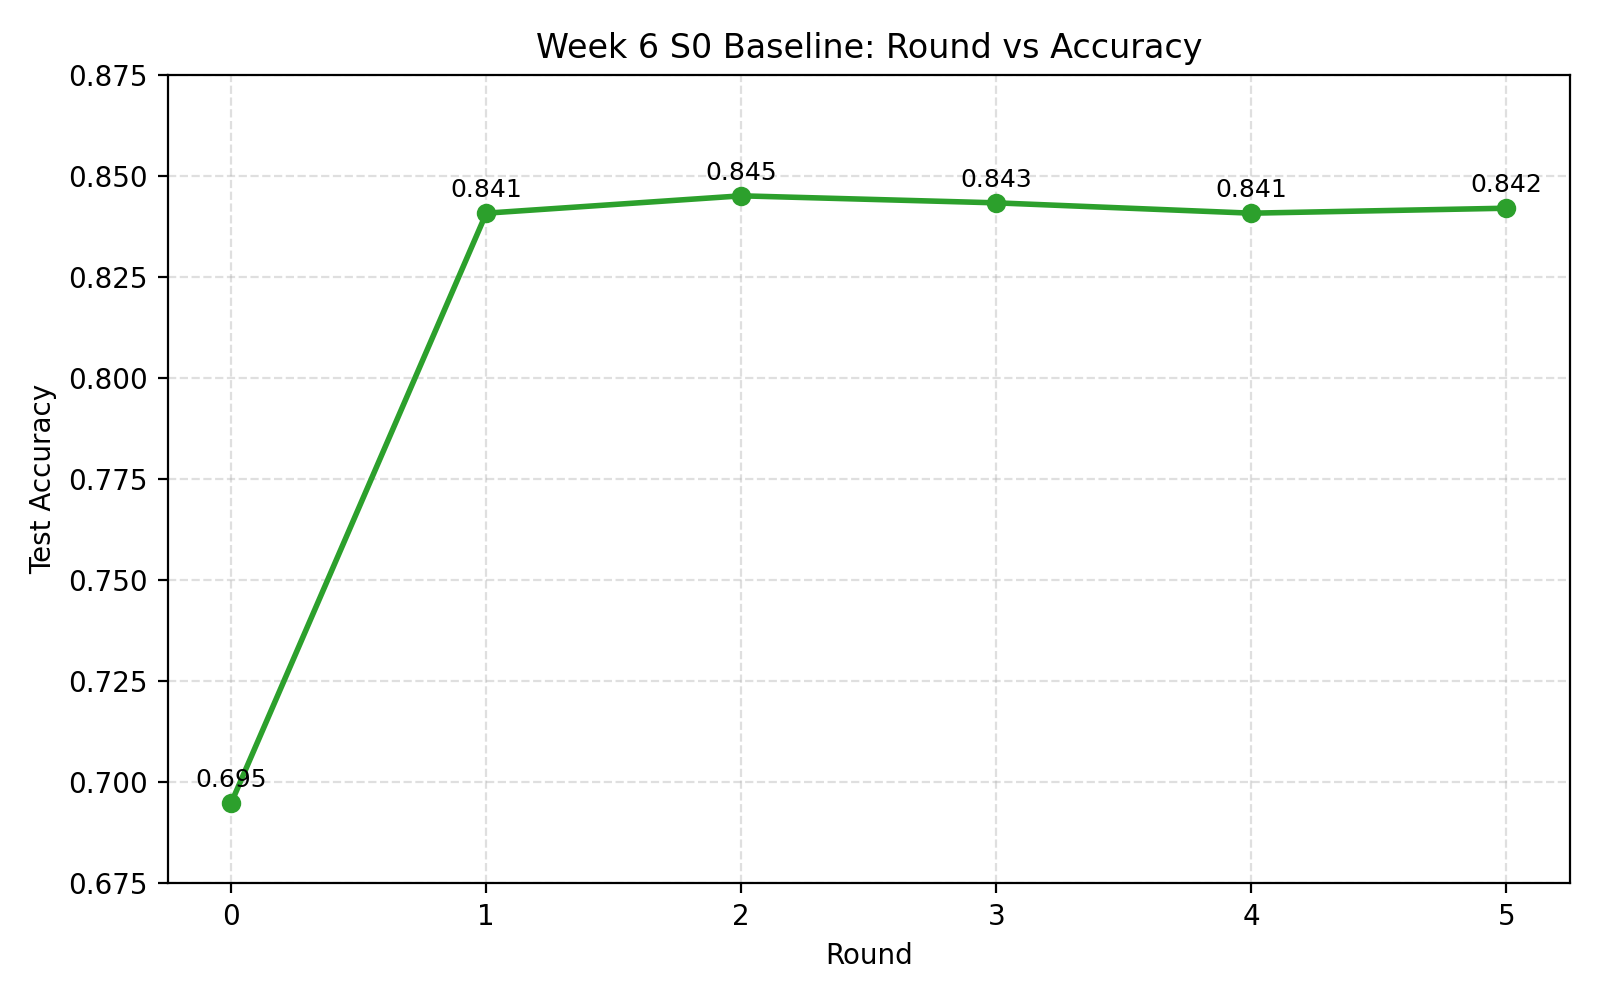
\includegraphics[width=0.62\linewidth]{round_vs_accuracy.png}
\caption{S0 FedAvg 基準在 Adult Income 上的逐輪準確率（$K=3$，5 輪）。}
\label{fig:s0}
\end{figure}

\subsection{量化約束、EZKL 實際證明與證明閘聚合（S2）}
\label{sec:res-constraint}
把裁剪與加性關係直接搬入整數約束時，誠實案例的裁剪上界在 $s\in\{100,1000,10000\}$ 下只有 5/9 精確成立、加性關係 0/9 精確成立（篡改案例 9/9 被拒絕）；浮點與量化關係的最大落差為 1 個單位，裁剪最大超額為 4200 ppm。這個觀察說明電路設計的主要風險不是抓不到惡意案例，而是誤拒合法案例。改用 canonical witness 後誠實關係 9/9 精確成立、篡改 9/9 拒絕；容差掃描得到可行區間 $(4200,\,73300)$ ppm，固定 4201 ppm 後推薦 profile 的誠實案例 9/9 通過、篡改 18/18 拒絕（表~\ref{tab:constraint}）。

\begin{table}[H]
\centering\small
\caption{約束條件由浮點到 canonical 量化見證的演進}
\label{tab:constraint}
\begin{tabular}{lccc}
\toprule
階段 & 誠實裁剪精確 & 誠實關係精確 & 篡改拒絕 \\
\midrule
直接量化浮點條件 & 5/9 & 0/9 & 9/9 \\
Canonical witness（無容差） & 5/9 & 9/9 & 9/9 \\
Canonical witness + 4201 ppm 容差 & 9/9 & 9/9 & 18/18 \\
\bottomrule
\end{tabular}
\end{table}

以 EZKL 對推薦 profile 建立檢查模型後，誠實案例 verified／clip／relation 全部為 True；篡改含噪更新雖仍能對其算術輸出產生有效證明，但關係殘差平方和為 1.0、relation 為 False，因而被閘拒絕。這區分了「證明檢查模型被正確計算」與「伺服器依公開輸出拒絕更新」兩個步驟。證明閘單輪實驗中 3 個客戶端有 2 個誠實更新被接受、1 個篡改更新被拒絕；把被接受的平均更新回寫全域模型後，下一輪準確率為 0.839697，未經閘的聚合為 0.836831（初始 0.694851）。單輪差距不能推廣為一般優勢，但顯示驗證結果已實際改變聚合結果。

\subsection{跨資料集效用：二元、多類別、大型與非同質}
\label{sec:utility}
表~\ref{tab:binary} 顯示 12 個二元資料集在預設參數下 9 個達到 90\% 保留率。Banknote、Blood Transfusion 與 Heart Disease 未達標；參數掃描後 Banknote（10 輪、噪聲 0.04）保留率 0.996970、Blood Transfusion（15 輪、噪聲 0.04）0.988201。依觀察歸因原則，這兩個資料集特徵維度極低（4 維）且基準本身不穩（FL 標準差 0.17／0.11），相同噪聲倍率造成較大的相對干擾，屬參數敏感而非方法不相容；報告保留原始未達標結果而不以調參後數字取代。Heart Disease 為提案承諾的資料集，以相同 pipeline 與預設參數補跑（線性模型，而非提案的 MLP）：303 筆是 12 個資料集中最小者，測試集僅 61 筆，FL 最終準確率 0.743169（標準差 0.033685），DP 為 0.617486（標準差 0.130004），保留率 0.830882；三個 seeds 中 seed 42 與 52 的 DP 準確率為 0.655738 與 0.754098，seed 62 跌至 0.442623，是拉低平均的主因。本研究未對 Heart Disease 另做參數掃描，直接保留此未達標結果。多類別 Iris／Wine／Digits 的保留率分別為 1.000000／1.009524／0.984586，Wine 略大於 1 反映 3 seeds 的隨機波動，不代表噪聲提升準確率。

\begin{table}[H]
\centering\small
\caption{12 個二元表格資料集的 FL/DP 最終準確率（3 seeds 平均；$K=3$、5 輪、$C=1.0$、噪聲 0.08）}
\label{tab:binary}
\begin{tabular}{lrrrrc}
\toprule
資料集 & 樣本數 & FL & DP & 保留率 & $\ge 90\%$ \\
\midrule
Banknote Authentication & 1,372 & 0.573333 & 0.467879 & 0.816067 & 否 \\
Blood Transfusion & 748 & 0.615556 & 0.535555 & 0.870036 & 否 \\
Breast Cancer Wisconsin & 569 & 0.912281 & 0.891813 & 0.977564 & 是 \\
German Credit & 1,000 & 0.711667 & 0.710000 & 0.997658 & 是 \\
Heart Disease（Cleveland） & 303 & 0.743169 & 0.617486 & 0.830882 & 否 \\
ILPD & 583 & 0.609687 & 0.601140 & 0.985981 & 是 \\
KC2 & 522 & 0.793651 & 0.784127 & 0.988000 & 是 \\
PC4 & 1,458 & 0.820776 & 0.794521 & 0.968011 & 是 \\
Pima Diabetes & 768 & 0.731602 & 0.714286 & 0.976332 & 是 \\
Spambase & 4,601 & 0.913138 & 0.907347 & 0.993658 & 是 \\
Tic-Tac-Toe & 958 & 0.656250 & 0.645833 & 0.984126 & 是 \\
Titanic & 1,309 & 0.821883 & 0.790076 & 0.961300 & 是 \\
\bottomrule
\end{tabular}
\end{table}

CoverType 大型資料實驗（表~\ref{tab:covertype}、圖~\ref{fig:covertype}）以 10,000、100,000 與完整 464,809 筆訓練分割、3 seeds、FL／clipping-only／DP 共 27 組配對執行。完整分割可在約 716 MiB 峰值 RSS、每次約 51 秒內完成；但效用並非隨資料量單調改善：完整分割的總落差 0.083091 中，clipping-only 落差 0.019257、噪聲額外落差 0.063834，保留率 0.884579 低於 90\% 門檻。這是由 control 得到的差距分解，不外推為一般因果比例。

\begin{table}[H]
\centering\small
\caption{Forest CoverType 訓練樣本量 scaling（3 seeds；$K=3$、5 輪）}
\label{tab:covertype}
\begin{tabular}{rrrrrrr}
\toprule
訓練樣本 & FL & Clip-only & DP & Clip/FL & DP/FL & 峰值 RSS (MiB) \\
\midrule
10,000 & 0.627299 & 0.627299 & 0.569942 & 1.000000 & 0.908566 & 599--607 \\
100,000 & 0.712285 & 0.701078 & 0.667886 & 0.984266 & 0.937666 & 598--627 \\
464,809 & 0.719890 & 0.700633 & 0.636799 & 0.973251 & 0.884579 & 715--716 \\
\bottomrule
\end{tabular}
\end{table}

\begin{figure}[H]
\centering
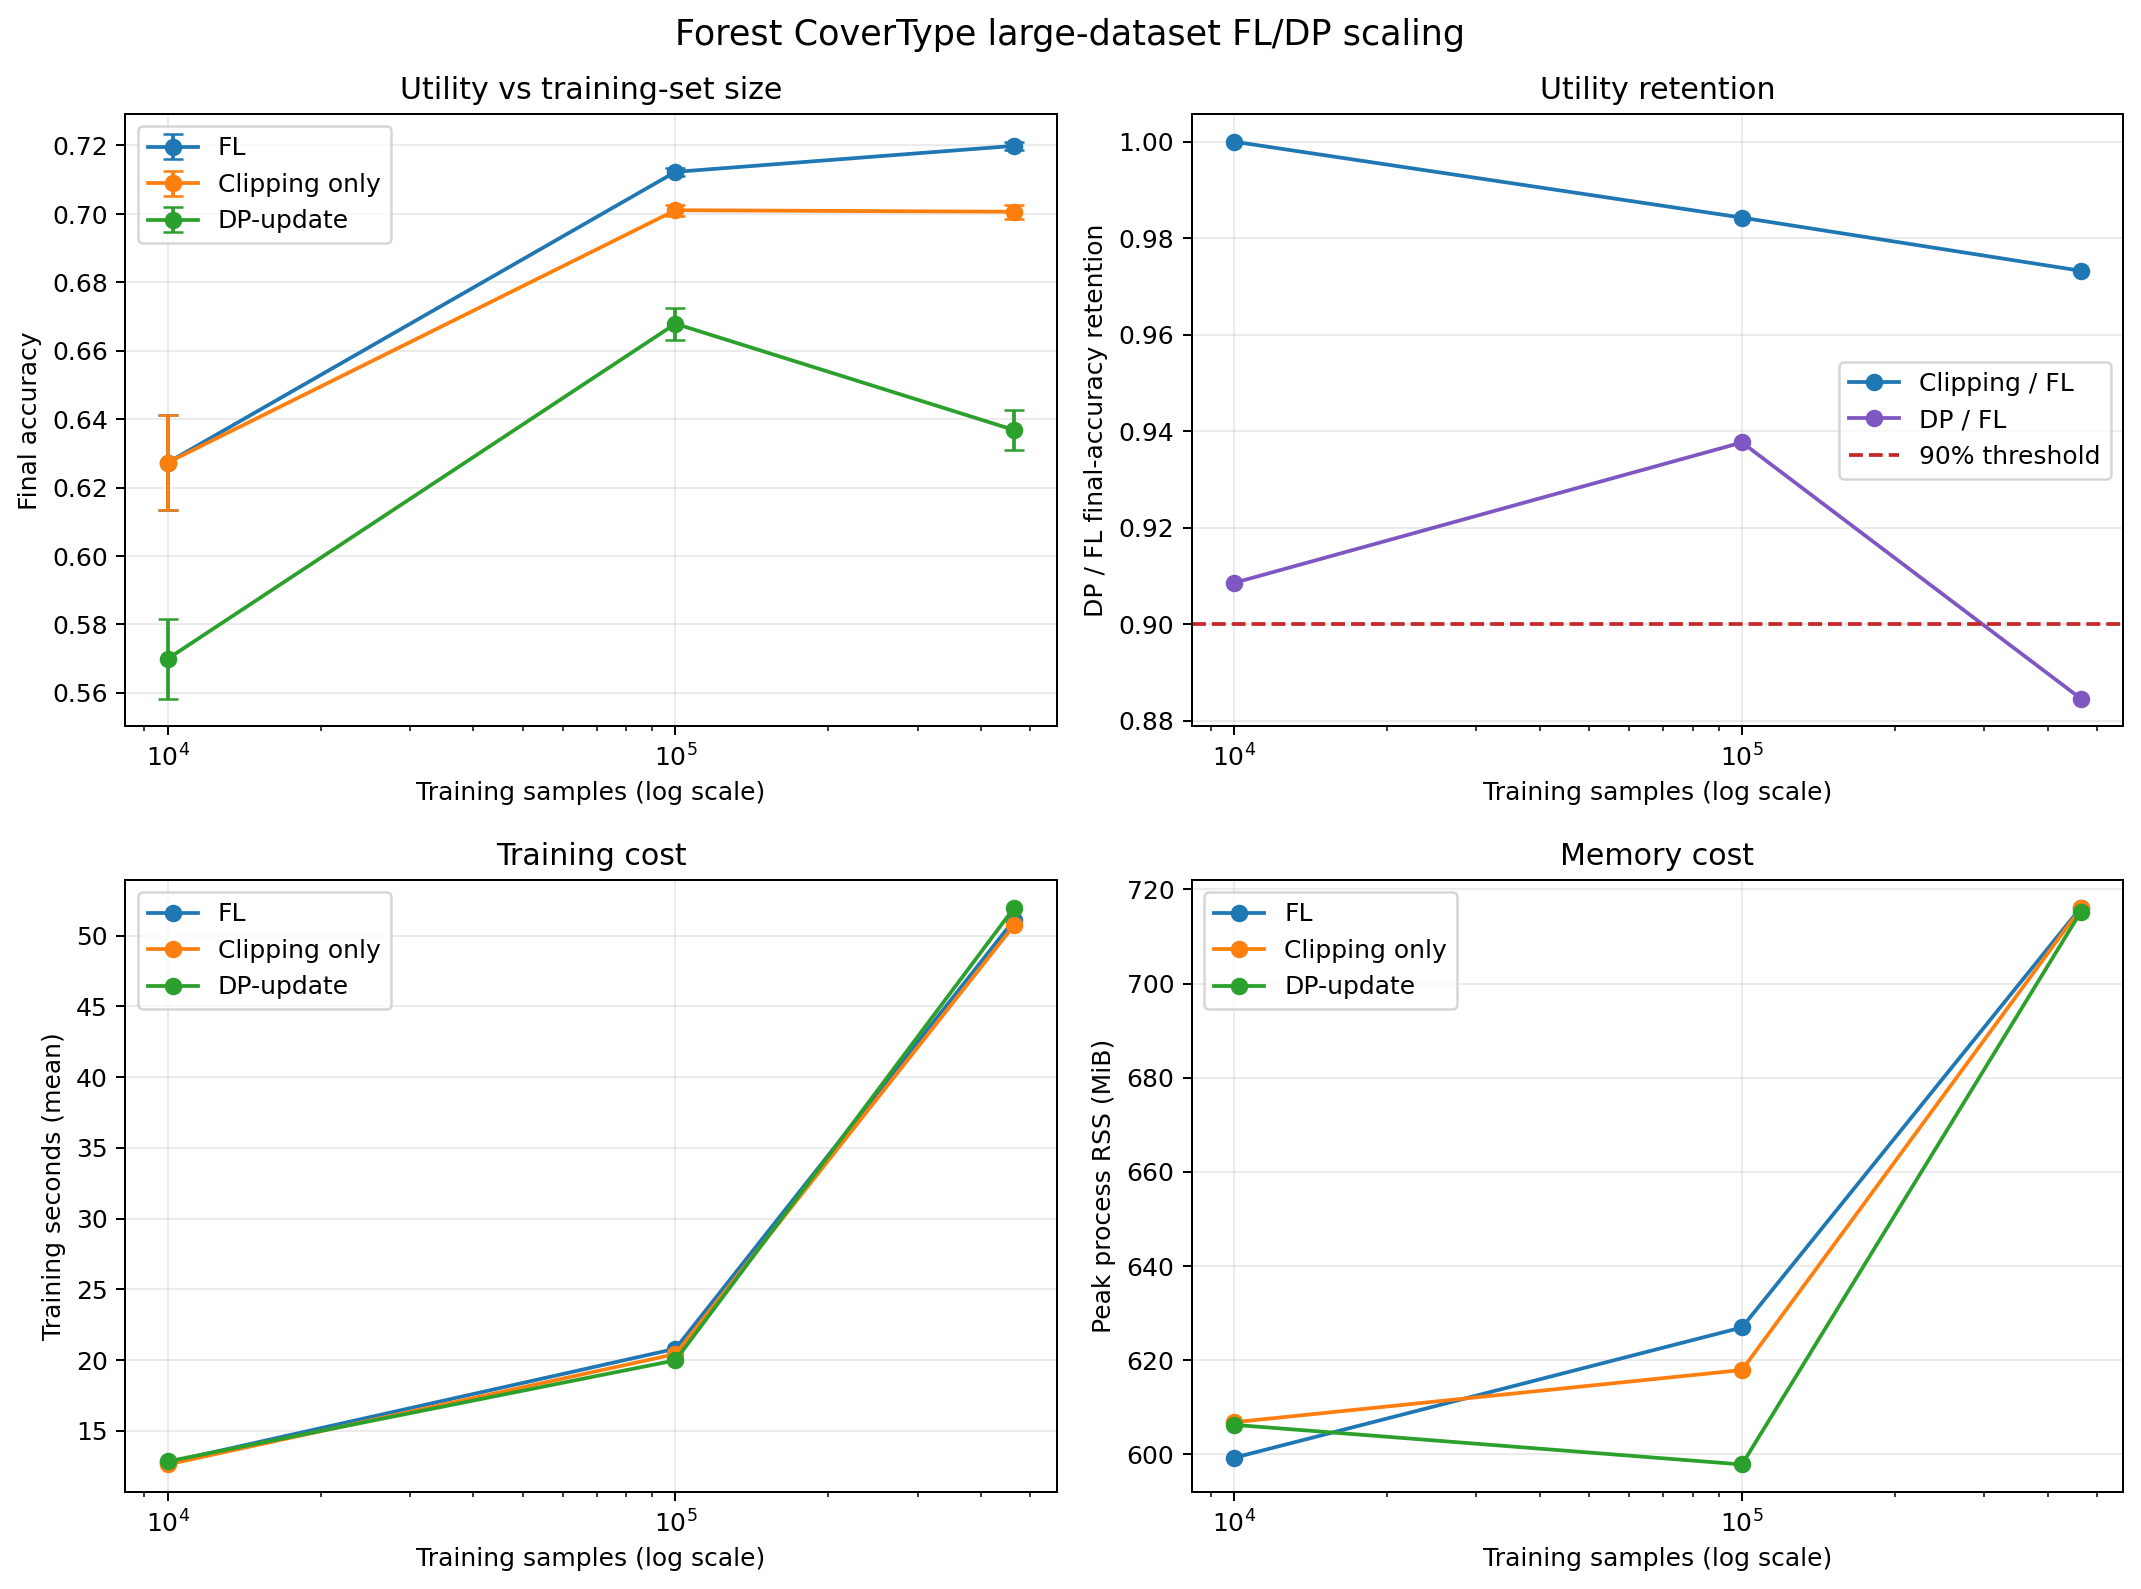
\includegraphics[width=0.9\linewidth]{covertype_scaling.png}
\caption{CoverType 大型資料 FL/DP scaling：效用、保留率、訓練時間與記憶體。}
\label{fig:covertype}
\end{figure}

非同質與客戶端數量實驗（表~\ref{tab:noniid}、圖~\ref{fig:noniid}）固定 100,000 筆、5 seeds，比較 $K=3/10$ 與 IID／Dirichlet $\alpha=0.5/0.1$，共 90 次模式執行。六個條件全部可執行，但 DP/FL 保留率從 $K=10$ IID 的 0.962019 降到 $K=3$、$\alpha=0.1$ 的 0.762431，且高度非同質條件的 CI 明顯變寬。結論是固定的裁剪／噪聲 profile 不具跨切分的效用穩健性，這是如實保留的負面結果。

\begin{table}[H]
\centering\small
\caption{CoverType 非同質與客戶端數量 scaling（5 seeds；100,000 筆；3 輪）}
\label{tab:noniid}
\begin{tabular}{rlrrrrr}
\toprule
$K$ & 切分 & Label TV & FL & DP & DP/FL & DP 95\% CI 半寬 \\
\midrule
3 & IID & 0.000 & 0.689464 & 0.612738 & 0.888716 & 0.012088 \\
3 & Dir. 0.5 & 0.282 & 0.679766 & 0.576464 & 0.848033 & 0.029448 \\
3 & Dir. 0.1 & 0.513 & 0.677091 & 0.516235 & 0.762431 & 0.068056 \\
10 & IID & 0.000 & 0.607950 & 0.584859 & 0.962019 & 0.026942 \\
10 & Dir. 0.5 & 0.369 & 0.630750 & 0.581477 & 0.921883 & 0.015131 \\
10 & Dir. 0.1 & 0.635 & 0.620605 & 0.518181 & 0.834961 & 0.058654 \\
\bottomrule
\end{tabular}
\end{table}

\begin{figure}[H]
\centering
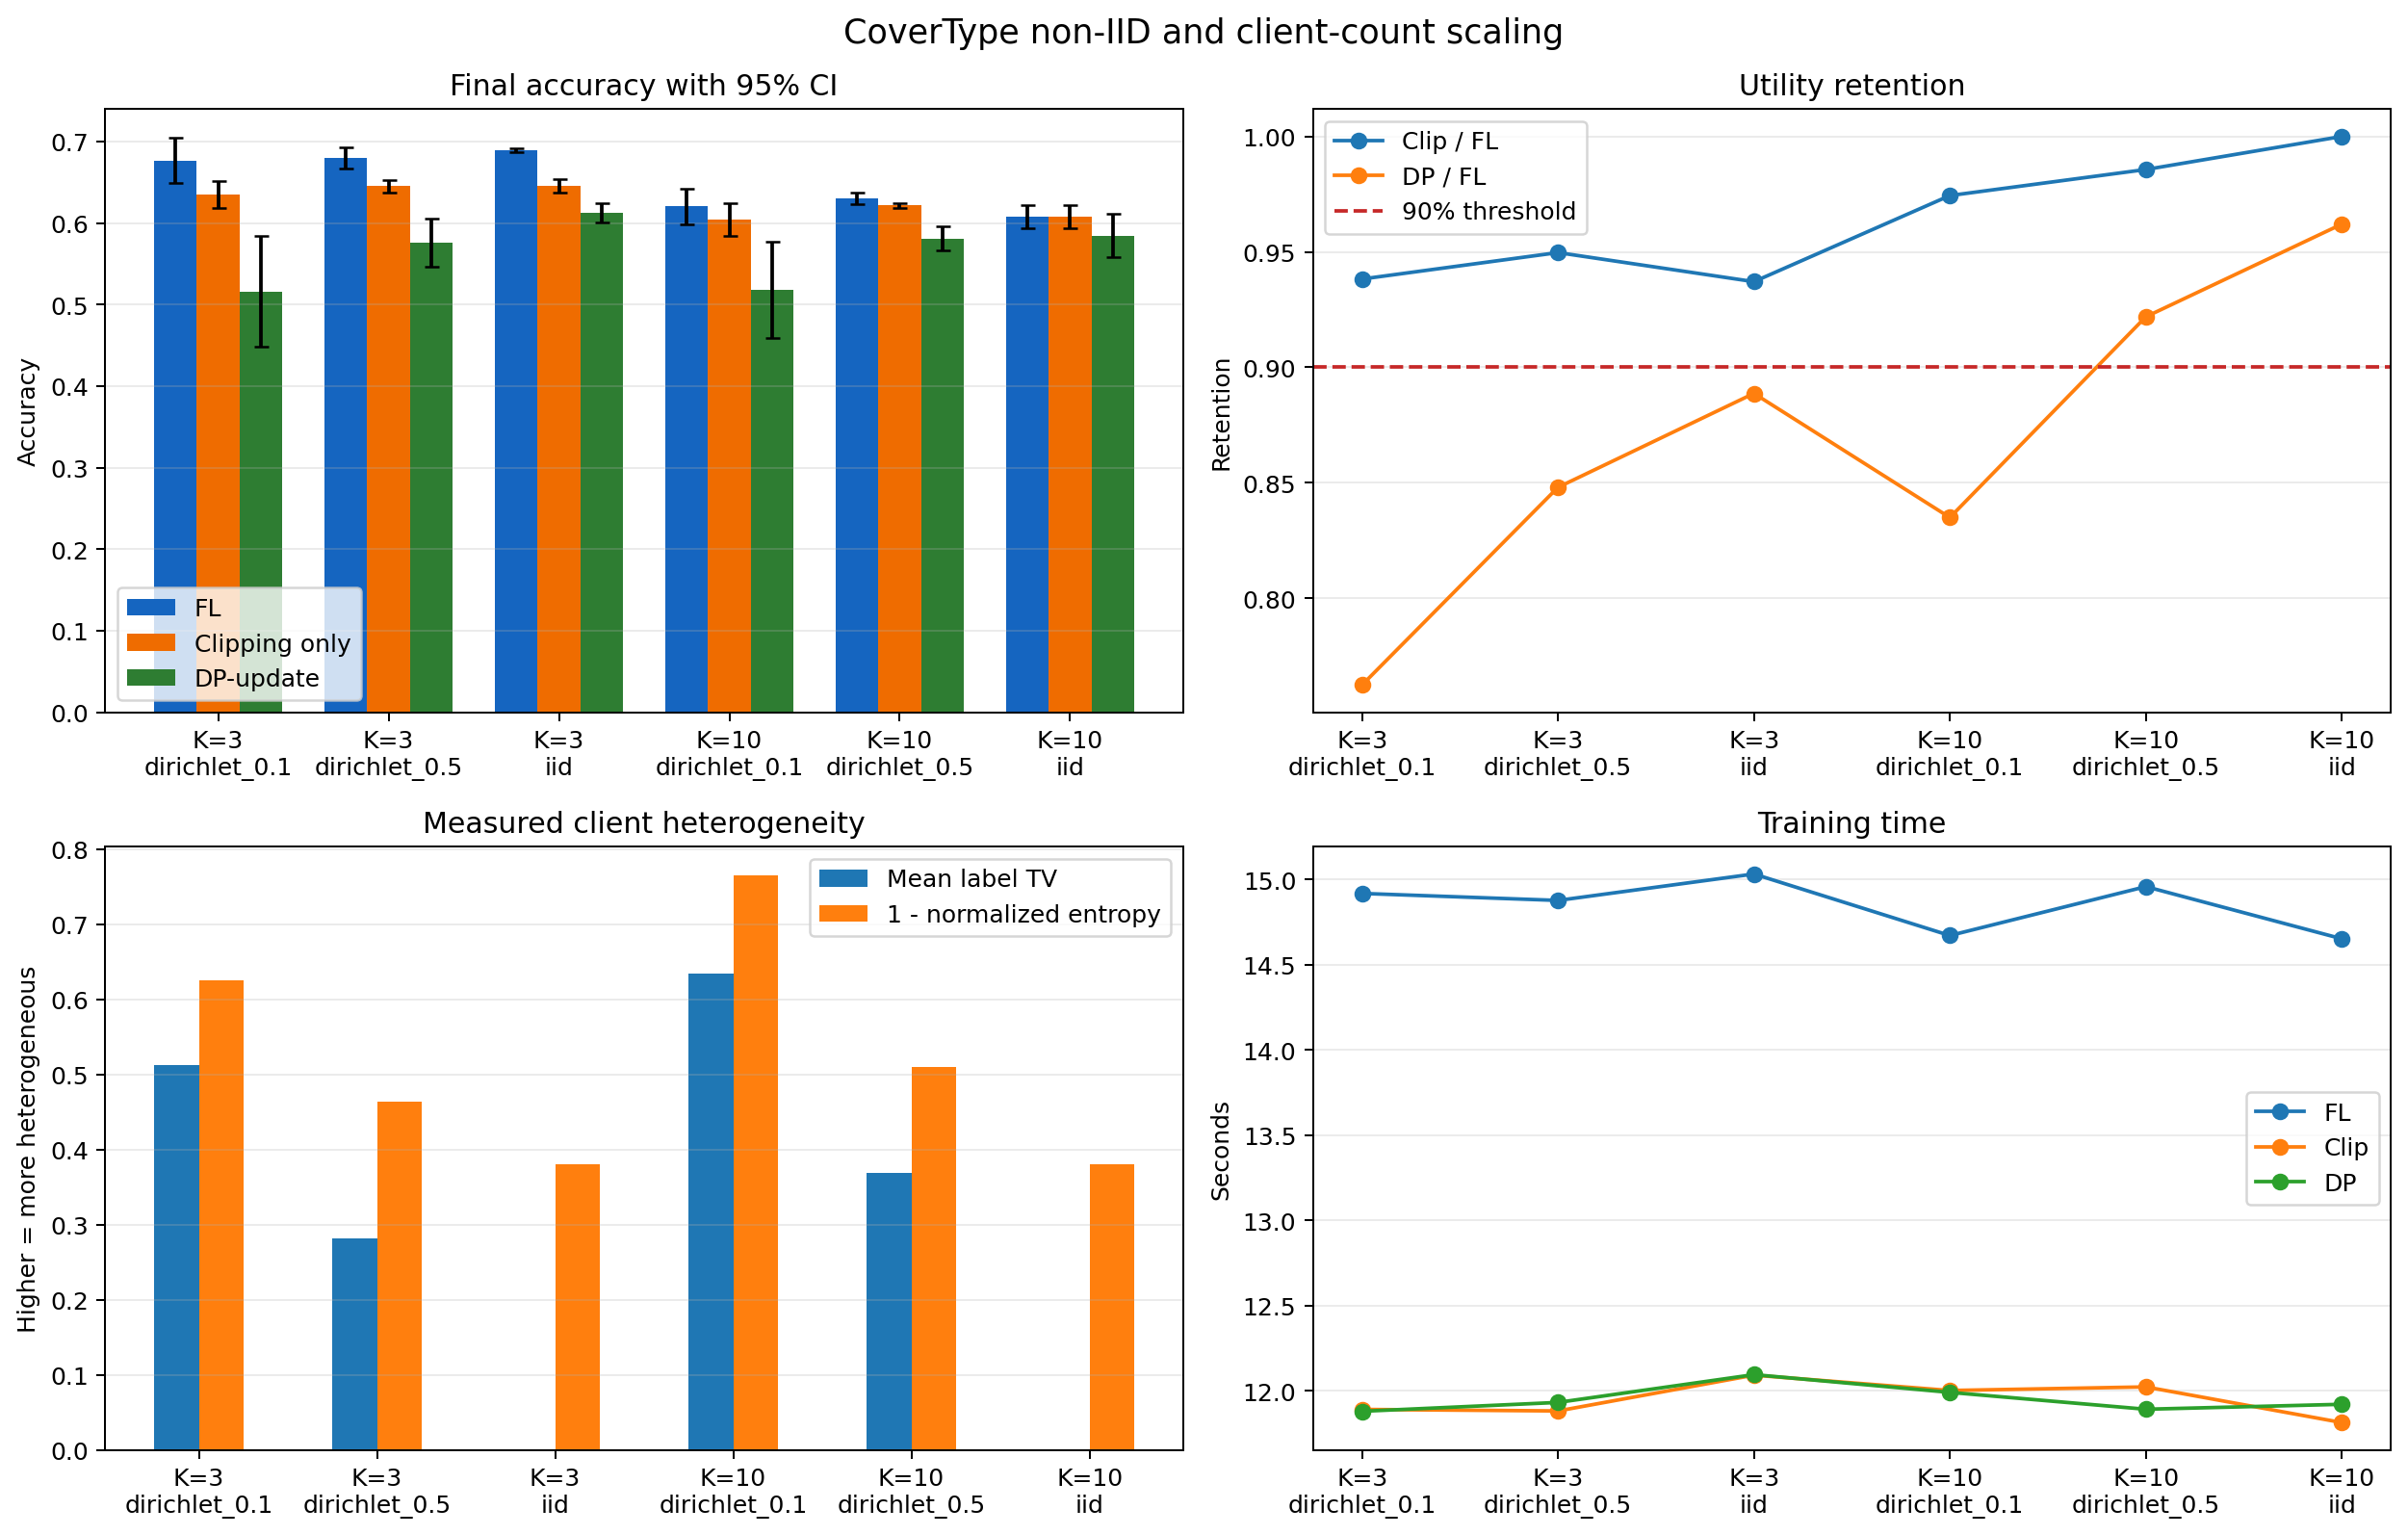
\includegraphics[width=0.9\linewidth]{noniid_client_scaling.png}
\caption{CoverType 非同質與客戶端數量 scaling：準確率、保留率、量測到的異質性與訓練時間。}
\label{fig:noniid}
\end{figure}

\subsection{零知識證明成本 scaling}
\label{sec:cost}
表~\ref{tab:cost} 彙整兩組 EZKL 實際證明：Iris／Wine／Digits 的完整 15／42／650 維更新，以及 CoverType 線性與 MLP 的 385／999／1,991 維更新，每組 3 seeds、誠實案例全數通過。維度由 15 增至 650 時，證明時間為 5.86 倍、電路列數由 138 增至 5,851、proving key 由 0.89 MB 增至 25.18 MB，而驗證時間與 proof 大小幾乎不變（圖~\ref{fig:cost}）。到 1,991 維時單一證明仍在 1.7 秒、峰值 RSS 471 MiB 內。這些數字落在本專題事先設定的綠色門檻內（證明 $\le 10$ 秒、RSS $\le 2$ GiB），但成長趨勢證實審查人指出的 scaling 風險；MLP 僅用於聯邦訓練，EZKL 只證明相同參數數量的更新向量約束，未把前向／反向傳播放入電路。

\begin{table}[H]
\centering\small
\caption{EZKL 完整更新向量約束證明的成本（誠實案例；3 seeds 平均，$\pm$ 為 95\% CI 半寬）}
\label{tab:cost}
\begin{tabular}{lrrrrrr}
\toprule
模型 & 維度 & Prove (s) & Verify (s) & Proof (B) & 電路列 & 峰值 RSS (MiB) \\
\midrule
Iris 線性 & 15 & 0.100 & 0.033 & 12,272 & 138 & 410.0 \\
Wine 線性 & 42 & 0.154 & 0.041 & 11,961 & 379 & 412.5 \\
Digits 線性 & 650 & 0.586 & 0.034 & 11,988 & 5,851 & 426.0 \\
CoverType 線性 & 385 & $0.530\pm0.136$ & $0.046\pm0.012$ & 12,268 & 3,468 & 419.1 \\
CoverType MLP-16 & 999 & $1.524\pm0.249$ & $0.054\pm0.005$ & 12,286 & 8,994 & 439.4 \\
CoverType MLP-32 & 1,991 & $1.658\pm0.431$ & $0.050\pm0.016$ & 12,282 & 17,922 & 471.3 \\
\bottomrule
\end{tabular}
\end{table}

\begin{figure}[H]
\centering
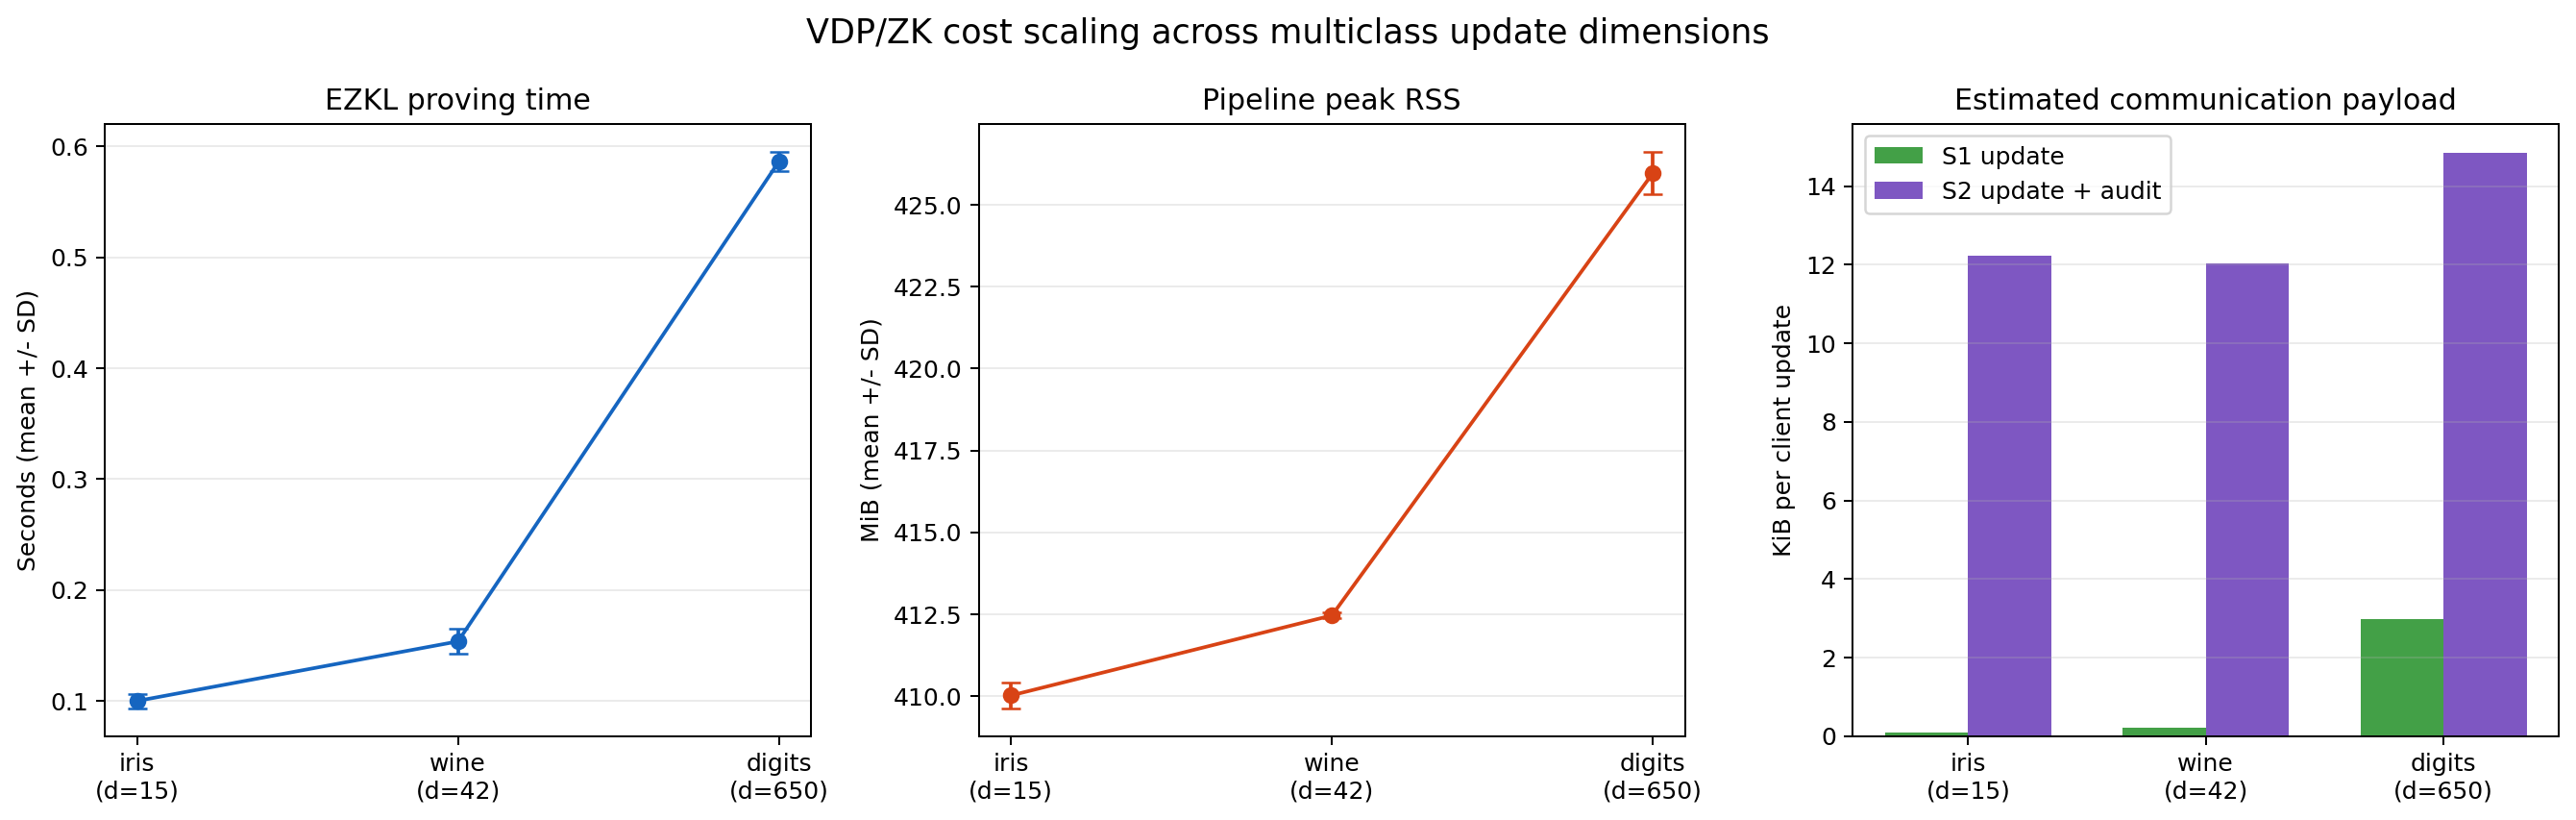
\includegraphics[width=0.95\linewidth]{zk_cost_scaling.png}
\caption{15／42／650 維更新的 EZKL 證明時間、峰值 RSS 與 application-layer 通訊負載。}
\label{fig:cost}
\end{figure}

聯邦訓練壓力測試（CoverType 50,000/20,000、Dirichlet 0.5、5 seeds）完成線性 $10\times3$、$25\times10$、$50\times20$ 與 MLP-16 $25\times10$ 共 40 條實際軌跡；clean 與 clipping + 二項式噪聲兩種模式的最終準確率相近（例如 $50\times20$ 為 $0.6384\pm0.0075$ 對 $0.6352\pm0.0108$）。以 385 維單一證明平均外推，$K=50$、$R=20$ 的 1,000 次更新若全部串行證明約需 0.147 小時、proof 約 11.70 MiB，而訓練本身只需約 27 秒：證明將是回合流程的主要成本，後續需金鑰重用、平行證明、部分參與或證明聚合。此外推值不是實際執行 1,000 份證明。

\subsection{秘密隨機性電路與逐更新多輪整合}
\label{sec:res-halo2}
Halo2 電路通過 8 個測試（4 個電路測試：誠實、篡改 $\qnoisy$、輪次情境替換、零噪聲偽造；4 個聯邦整合測試：JSON 位元精確往返、失敗消耗 ticket、資料相依訓練落在電路範圍、模型綁定與 accepted-only 聚合）。10 個獨立 seeds 的實際證明 10/10 通過、proof 雜湊 10/10 唯一，每份 3,840 bytes，證明 $1.8452\pm0.0407$ 秒、驗證 $0.0619\pm0.0091$ 秒、峰值 RSS $246.21\pm0.74$ MiB。GitHub Actions 在 Ubuntu 與 Windows 各自重現 3 份證明與 2 客戶端 × 2 輪軌跡，最近一次（2026-10-05）全部通過。

逐更新多輪整合（表~\ref{tab:multiround}、圖~\ref{fig:multiround}）在 5 seeds × 3 客戶端 × 10 輪上為每一份更新產生實際 IPA 證明，只聚合通過者，並由獨立程序從磁碟重新產生驗證金鑰、重驗全部證明與模型鏈。150/150 證明通過、150/150 磁碟重驗、5/5 模型鏈完整；每份證明以 7 種探測（重播、客戶端／輪次／模型替換、含噪更新篡改、證明位元組損壞、失敗後重試）測試，1,050/1,050 被拒絕，其中重播的原始證明仍能通過密碼學驗證，必須由伺服器 ticket 狀態拒絕。所有誠實回合中，證明閘與相同含噪更新的直接聚合差異為 0（算術一致性檢查）。噪聲帶來的效用代價明顯：證明閘含噪最終準確率 $0.8309\pm0.0989$，無噪聲量化訓練 $0.9441\pm0.0148$；seed 62 僅 0.707，反映 $k=16$ 噪聲對 $\pm1$ 量化 4 維更新的相對幅度很大。

\begin{table}[H]
\centering\small
\caption{逐更新 Halo2 多輪整合（3 客戶端 × 10 輪 × 5 seeds；$\pm$ 為以軌跡為單位的 95\% CI 半寬）}
\label{tab:multiround}
\begin{tabular}{lr}
\toprule
指標 & 實測 \\
\midrule
實際產生且通過的證明 & 150/150 \\
磁碟重驗 & 150/150（唯一雜湊 150） \\
完整模型鏈 & 5/5 \\
負面探測拒絕 & 1,050/1,050 \\
每更新證明／驗證秒數 & $1.9520\pm0.7963$ ／ $0.0450\pm0.0201$ \\
每軌跡 wall 秒數／峰值 RSS & $73.21\pm28.68$ s ／ $238.51\pm0.65$ MiB \\
證明閘含噪最終準確率 & $0.8309\pm0.0989$ \\
無噪聲量化對照準確率 & $0.9441\pm0.0148$ \\
\bottomrule
\end{tabular}
\end{table}

\begin{figure}[H]
\centering
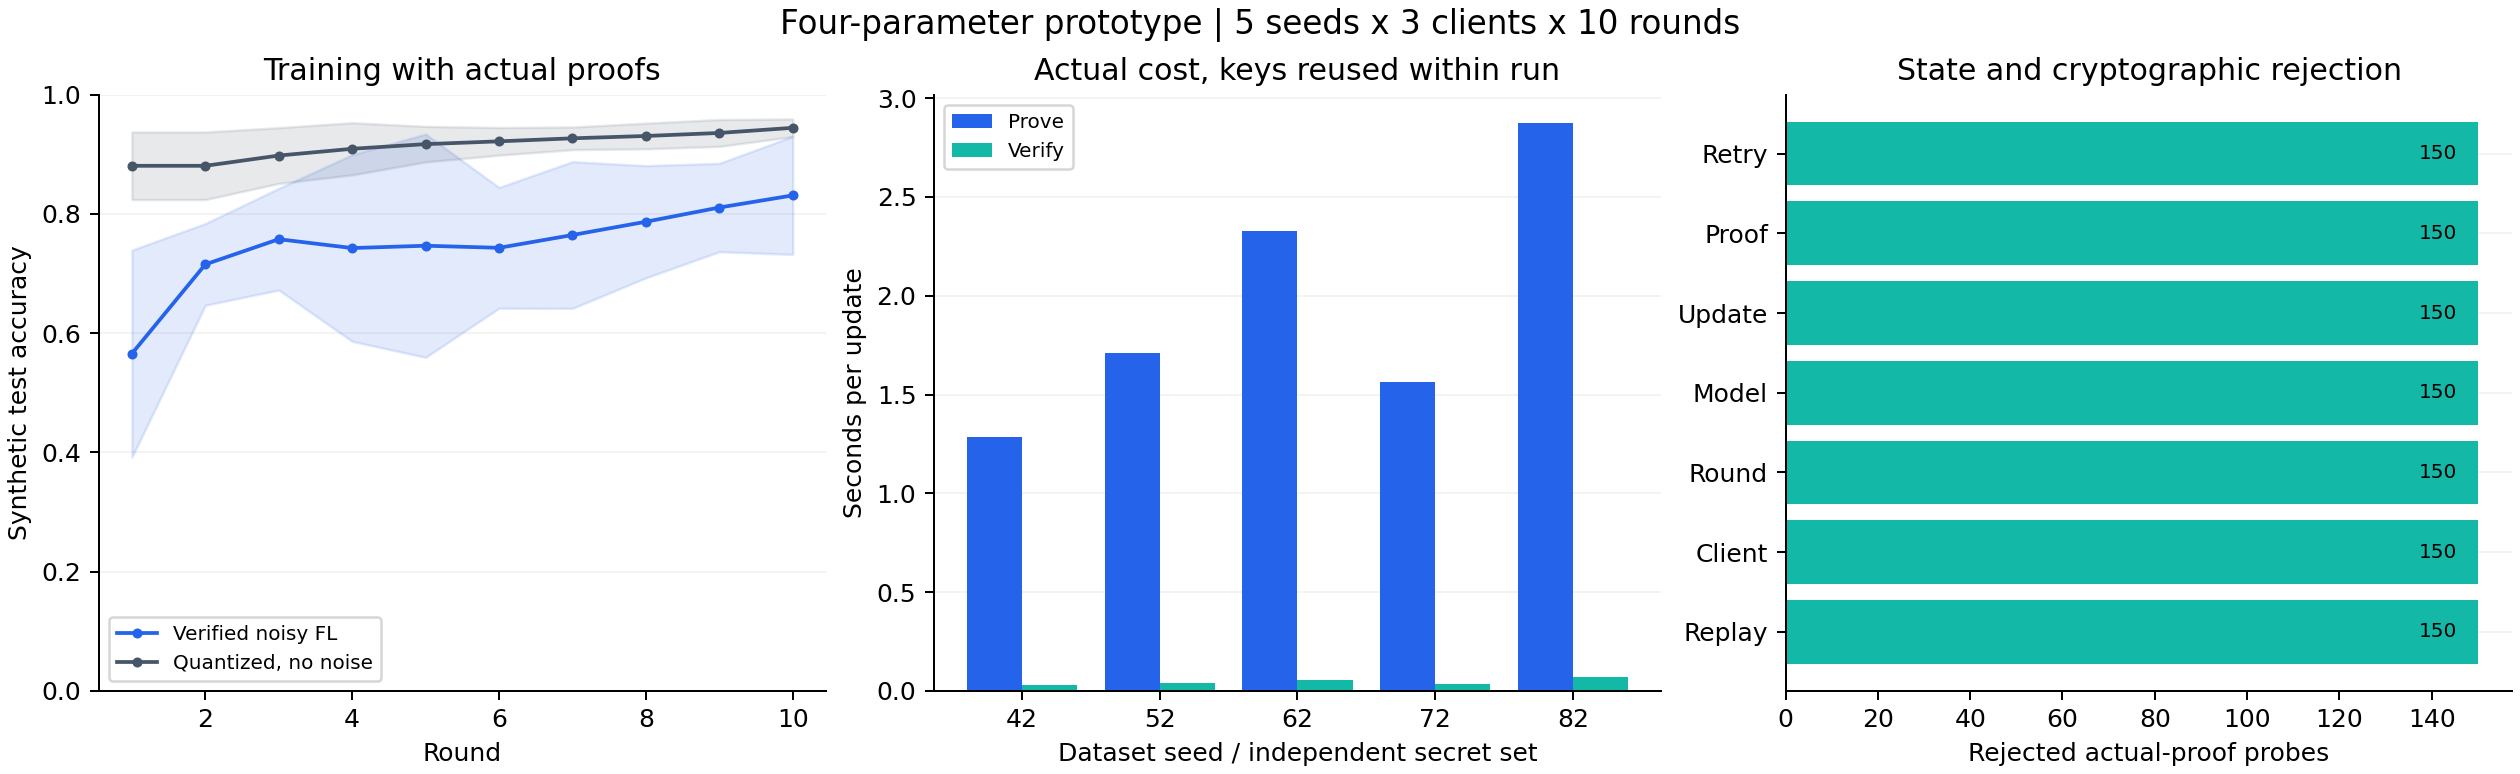
\includegraphics[width=0.98\linewidth]{multiround_halo2.png}
\caption{4 參數原型：含實際證明的訓練曲線、各 seed 的證明／驗證成本，以及 7 類負面探測的拒絕計數。}
\label{fig:multiround}
\end{figure}

一個保留的失敗紀錄：初次 pilot 的 30 份證明即時驗證成功，但模型由 JSON 讀回時一個數值相差 1 ULP（$-6.938893903907228\times10^{-17}$ 變為 $\ldots227\times10^{-17}$），導致精確模型鏈核對失敗。修正方式是啟用 serde\_json 的 float\_roundtrip 並加入位元精確回歸測試，而非放寬模型雜湊容差；修正後同批 pilot 重驗成功，再以全新 OS 隨機材料重跑正式矩陣。

\subsection{隱私預算：負面結果與固定 profile 的有限 $\eps$}
\label{sec:privacy}
\textbf{公開種子的負面結果。}S1／EZKL 線的 artifact 把確定性噪聲種子列為公開輸入；驗證者可重建 $\qnoise$ 並由 $\qnoisy-\qnoise$ 還原 $\qclip$，因此驗證者視角的隱私預算為 $\eps=\infty$。即使假設改用驗證者不知道的獨立 Gaussian 噪聲，client-level R\'enyi DP 會計~\cite{mironov2017rdp}（$q=1$、replace-one 敏感度 $2C$、10 輪、$\delta=10^{-5}$）顯示現行噪聲倍率 0.08 的條件式 $\eps$ 仍為 3504.357；要達到 $\eps=128/32/8$ 分別需要倍率 $0.531/1.396/4.366$，而三個多類別資料集的保留率隨之跌破 90\%（表~\ref{tab:frontier}、圖~\ref{fig:frontier}）。這說明「可驗證加噪」與「可驗證且不可預測的 DP 隨機性」是兩個不同問題，也說明高效用與有意義隱私預算之間存在實質衝突。

\begin{table}[H]
\centering\small
\caption{條件式（秘密 Gaussian 假設）replace-one $\eps$ 與保留率；公開種子現況為 $\eps=\infty$}
\label{tab:frontier}
\begin{tabular}{lrrrr}
\toprule
資料集 & 噪聲 0.08（$\eps=3504.357$） & $\eps=128$ & $\eps=32$ & $\eps=8$ \\
\midrule
Digits & 0.984586 & 0.536609 & 0.252409 & 0.171483 \\
Iris & 1.000000 & 0.782051 & 0.500000 & 0.384615 \\
Wine & 1.009524 & 0.876190 & 0.609524 & 0.457143 \\
\bottomrule
\end{tabular}
\end{table}

\begin{figure}[H]
\centering
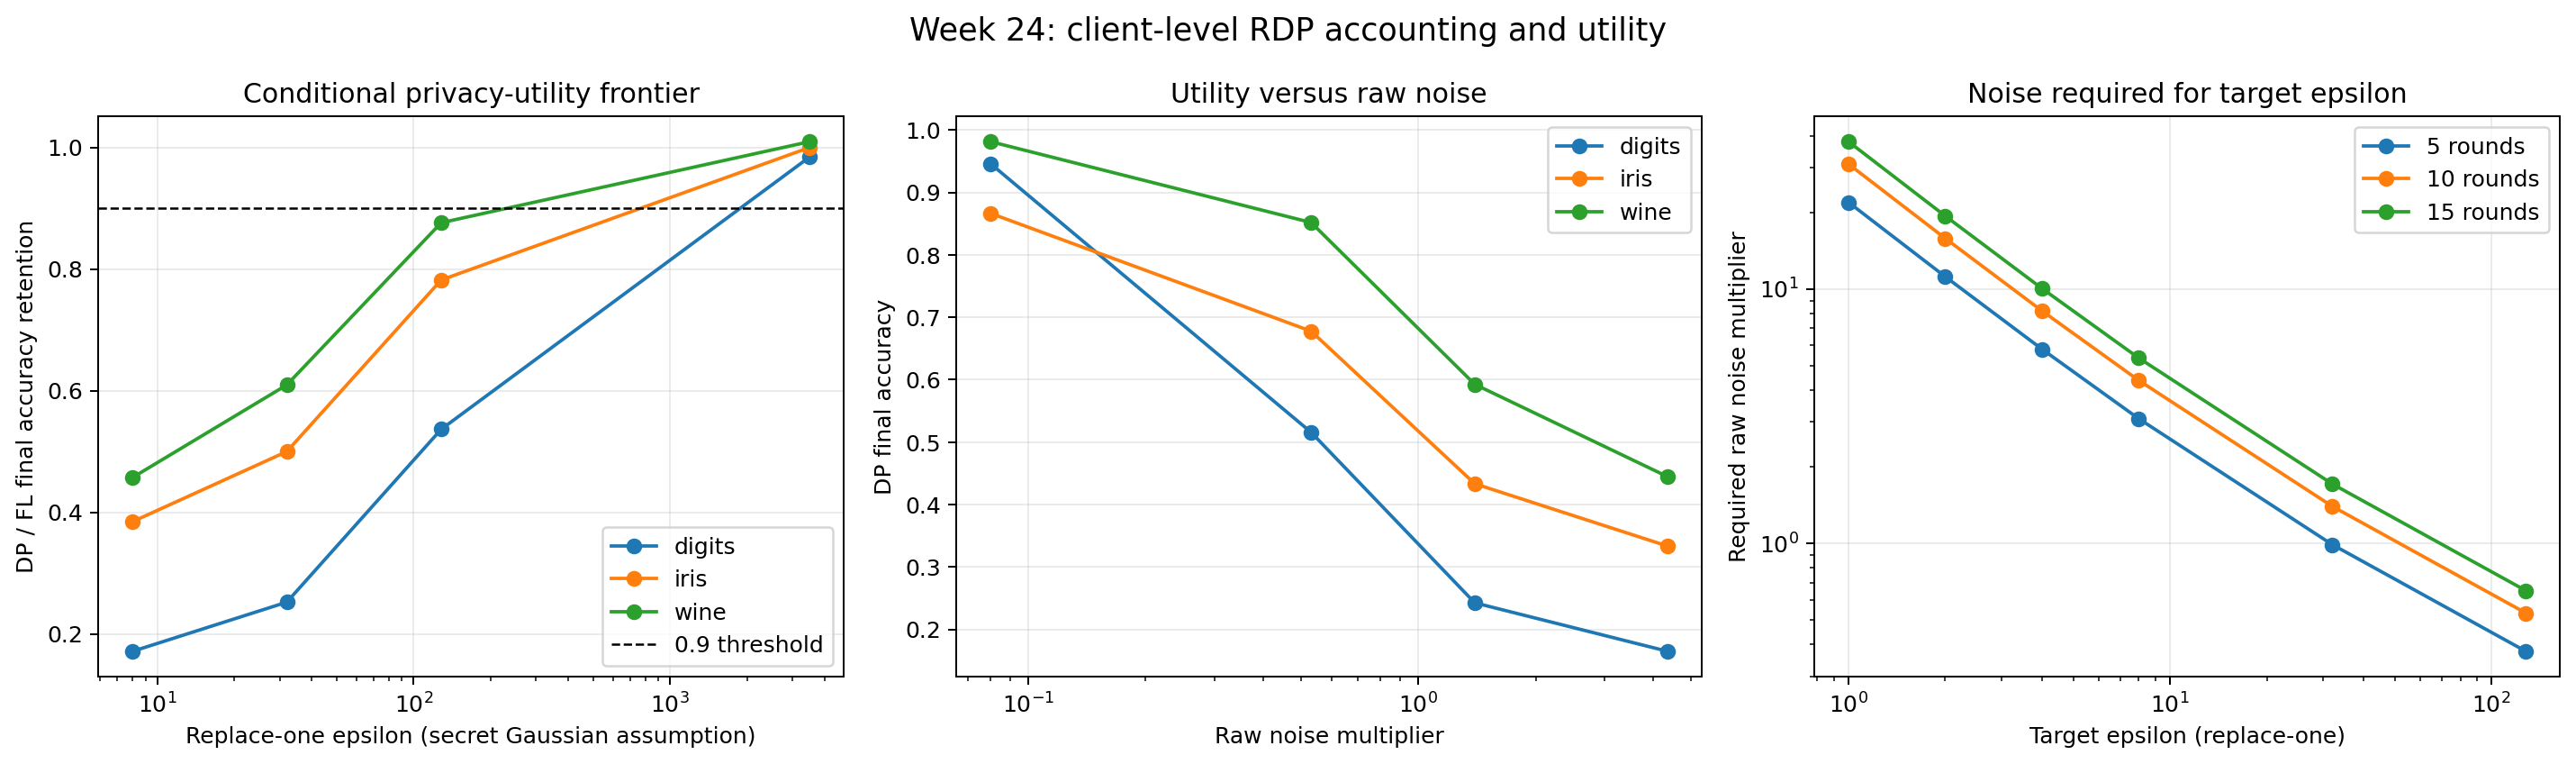
\includegraphics[width=0.98\linewidth]{privacy_utility_frontier.png}
\caption{條件式 client-level RDP 會計下的隱私—效用前緣、效用對原始噪聲倍率，以及目標 $\eps$ 所需噪聲。}
\label{fig:frontier}
\end{figure}

\textbf{固定 profile 的有限 $\eps$。}對 Halo2 線的理想離散機制，exact PLD 會計得到表~\ref{tab:accountant} 的結果：$d=4$、$k=16$、10 輪（40 次標量組合）、$\delta=10^{-5}$ 時 $\eps\le 28.840669$，不可避免的 $\delta$ 下限 $3.07\times10^{-7}$，域低位元偏差上界 $5.9\times10^{-66}$。$k=32/64$ 可把 $\eps$ 降至 17.98／11.54，但電路位元與約束隨之增加；200 次組合（$k=32$）時 $\eps$ 升至 54.71，顯示輪數與維度仍是隱私瓶頸。另以精確有理數計算的保守基本組合上界為 195.85；它是較鬆的診斷值，與 PLD 的 28.84 不矛盾，也不是實測隱私惡化。若把 $k=16$ 直接延伸到 385 或 1,991 維且每座標仍允許 $\pm1$，$\delta$ 下限（$5.9\times10^{-5}$、$3.1\times10^{-4}$）已超過 $10^{-5}$，無法取得有限 $\eps$；這也是高維 EZKL 線不繼承四維定理的原因。

\begin{table}[H]
\centering\small
\caption{Exact centered-binomial PLD 會計（replacement client-level，位移 2，$\delta=10^{-5}$）}
\label{tab:accountant}
\begin{tabular}{rrrrr}
\toprule
$k$ & 組合次數 & $\eps$ 上界 & $\delta$ 下限 & 域位元偏差 \\
\midrule
16 & 40 & 28.840669 & $3.07\times10^{-7}$ & $5.9\times10^{-66}$ \\
32 & 40 & 17.979538 & $1.41\times10^{-16}$ & $2.5\times10^{-56}$ \\
64 & 40 & 11.541361 & $1.52\times10^{-35}$ & $4.7\times10^{-37}$ \\
32 & 200 & 54.709923 & $7.05\times10^{-16}$ & $1.3\times10^{-55}$ \\
\bottomrule
\end{tabular}
\end{table}

必須強調 $\eps=28.84$ 仍是很大的預算，不應描述為強實務隱私；而且此定理只對理想取樣器與固定參與排程成立，完整 transcript（承諾、證明、時間、重試）的 DP 仍需審查 commitment hiding、PRF/ZK simulation 與適應性組合。

\subsection{多輪威脅矩陣與穩健聚合}
\label{sec:threatmatrix}
為界定閘的保證邊界，多輪威脅矩陣（CoverType 100,000 筆、$K=10$、Dirichlet 0.1、3 輪、20\% 攻擊者、3 seeds）對 5 種攻擊比較 ungated、current gate（proof + clip + relation）與 strengthened gate（加情境綁定、重播保護、噪聲生成政策），共 48 條軌跡與 1,440 次客戶端決策（表~\ref{tab:threat}、圖~\ref{fig:threat}）。這 1,440 次決策重用前述 actual-EZKL 的 artifact／check contract，是政策模擬，不是 1,440 份實際證明。

\begin{table}[H]
\centering\small
\caption{多輪 proof-gated 威脅矩陣（clean DP 最終準確率 0.495314）}
\label{tab:threat}
\begin{tabular}{lrrrr}
\toprule
 & \multicolumn{2}{c}{惡意更新接受率} & \multicolumn{2}{c}{Clean 保留率} \\
\cmidrule(lr){2-3}\cmidrule(lr){4-5}
攻擊 & Current & Strengthened & Current & Strengthened \\
\midrule
Relation tamper & 0.00 & 0.00 & 0.585848 & 0.585848 \\
Clip bypass & 0.00 & 0.00 & 0.585848 & 0.585848 \\
Replay & 1.00 & 0.00 & 0.975868 & 0.718373 \\
Zero noise & 1.00 & 0.00 & 1.197807 & 0.585848 \\
Bounded sign flip & 1.00 & 1.00 & 0.179797 & 0.179797 \\
\bottomrule
\end{tabular}
\end{table}

\begin{figure}[H]
\centering
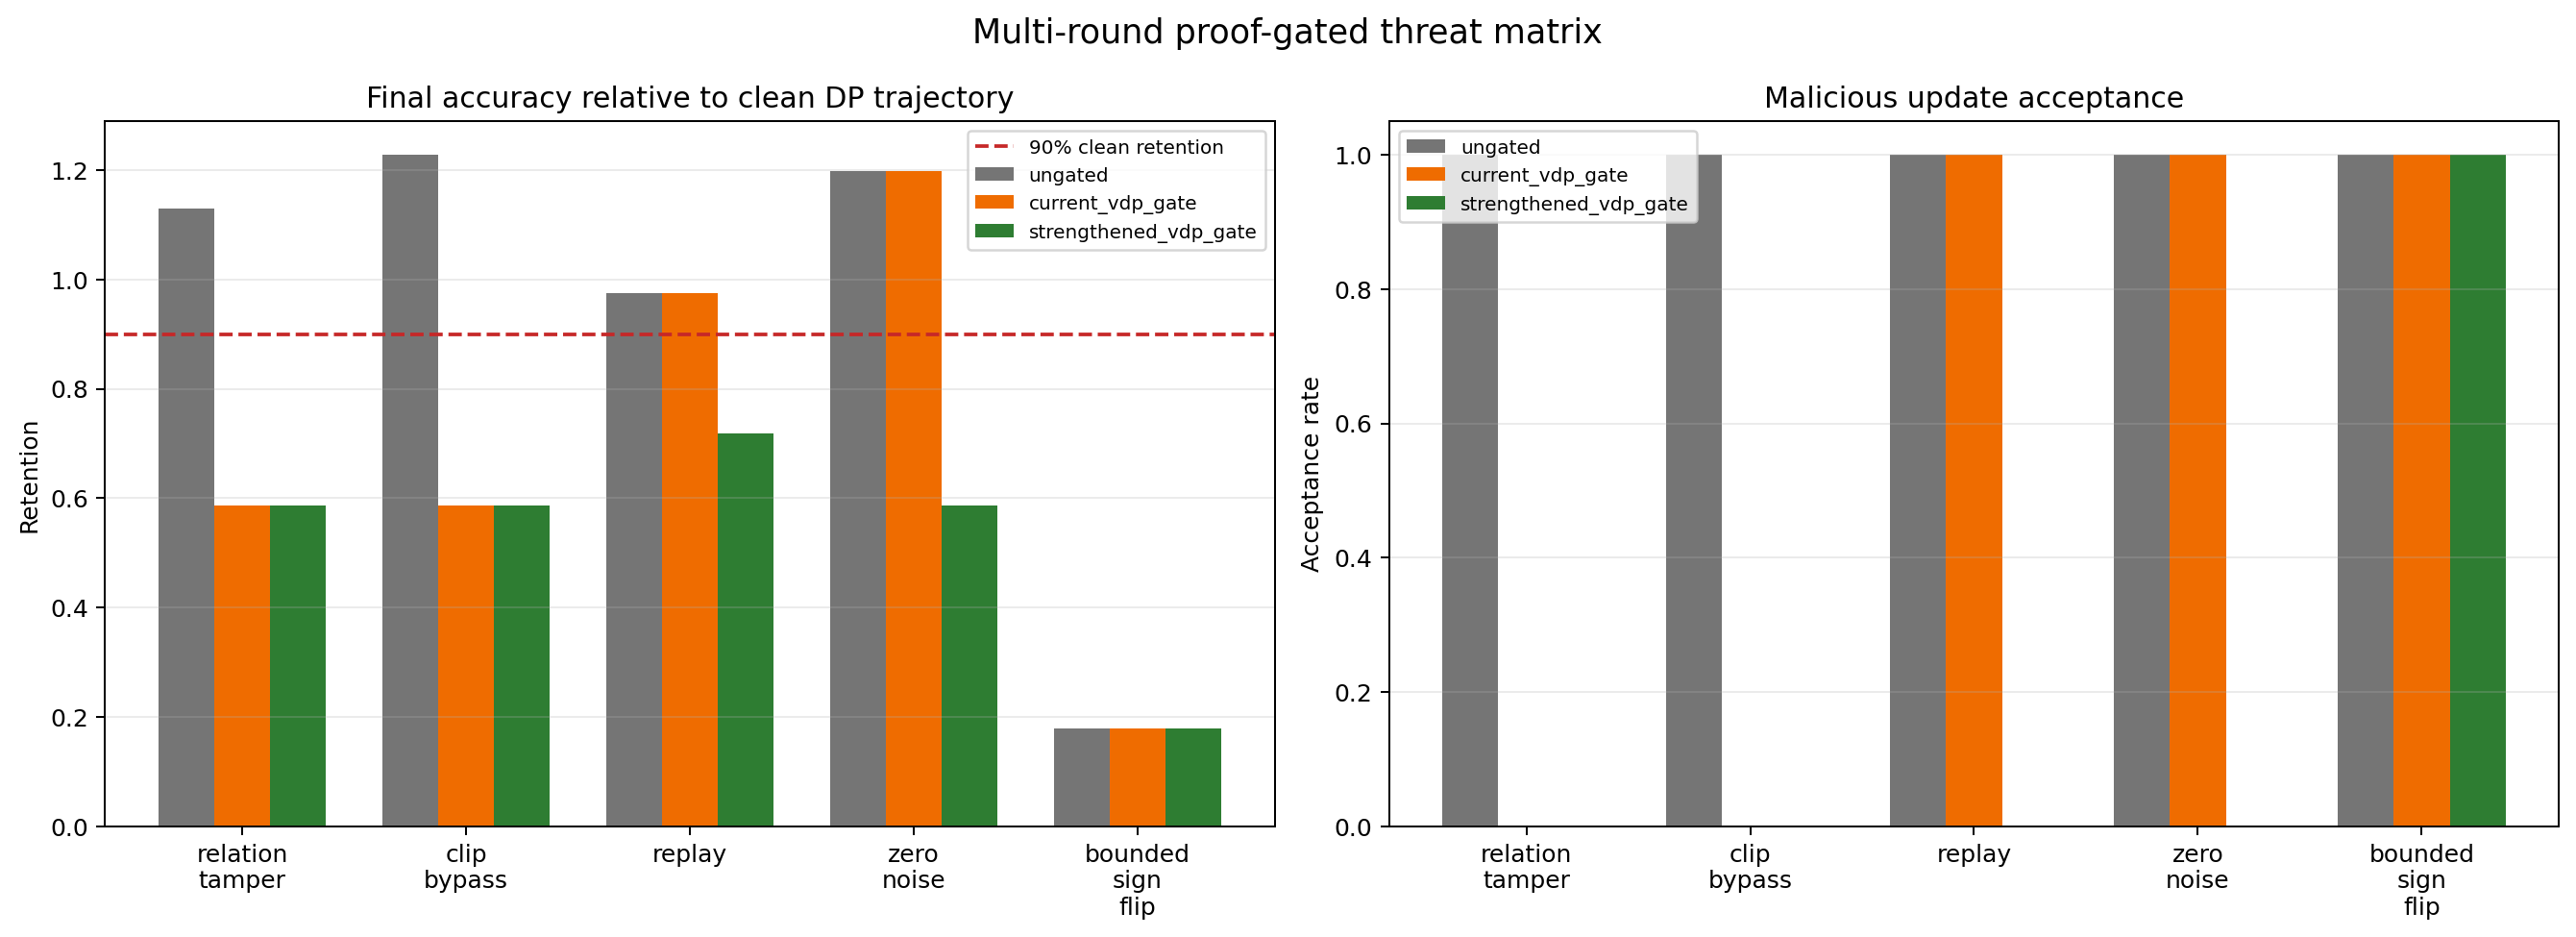
\includegraphics[width=0.95\linewidth]{threat_matrix.png}
\caption{多輪威脅矩陣：相對 clean DP 軌跡的最終準確率，以及三種政策下的惡意更新接受率。}
\label{fig:threat}
\end{figure}

結果支持三個精確結論。第一，current gate 對其聲明範圍內的 relation／clip 違規在多輪情境下確實拒絕（接受率 0\%）。第二，僅驗證加性關係不足以阻擋重播與零噪聲（接受率 100\%）；加入情境與噪聲生成政策後降為 0\%，這正是第~\ref{sec:halo2} 節 Halo2 電路要解決的缺口。第三，合法裁剪範圍內的符號反轉更新在所有政策下 100\% 通過，clean 保留率僅 0.179797：更新層級的 VDP 閘不能被誇大為本地訓練正確性或任意投毒防禦。兩個需要解釋的現象是：zero-noise 與 clip-bypass 在 ungated 下保留率大於 1，因為移除噪聲或放大更新會提高準確率，所以「準確率上升」不能當作安全訊號；拒絕兩個最大的非同質客戶端後 strengthened 軌跡的 clean 保留率只有 0.585848，揭露安全拒絕與可用資料之間的代價。

穩健聚合實驗（CoverType 50,000/20,000、$K=10$、$R=5$、Dirichlet 0.5、20\% 攻擊者、10 seeds）中攻擊者提交反向並放大至裁剪上界的合法更新，3,000/3,000 次決策（含 300/300 惡意更新）全部通過 strengthened gate。相較均值，座標中位數的配對保留率增益為 $0.1988\pm0.0404$、截尾平均 $0.1541\pm0.0306$，two-sided exact sign-flip $p=0.001953$（表~\ref{tab:robust}）。這是本研究唯一可稱「顯著」的比較，但中位數／截尾平均的攻擊下保留率仍只有約 0.59／0.54，不能寫成完全防禦。

\begin{table}[H]
\centering\small
\caption{20\% 合法範圍投毒下的穩健聚合（10 seeds；$\pm$ 為 95\% CI 半寬）}
\label{tab:robust}
\begin{tabular}{lrrrr}
\toprule
聚合器 & Clean 準確率 & 攻擊下準確率 & 配對變化 & 攻擊／clean 保留率 \\
\midrule
均值 & $0.6012\pm0.0096$ & $0.2327\pm0.0269$ & $-0.3685\pm0.0249$ & $0.3867\pm0.0430$ \\
座標中位數 & $0.5911\pm0.0100$ & $0.3463\pm0.0376$ & $-0.2448\pm0.0350$ & $0.5855\pm0.0606$ \\
截尾平均 & $0.5980\pm0.0103$ & $0.3237\pm0.0309$ & $-0.2743\pm0.0275$ & $0.5408\pm0.0480$ \\
\bottomrule
\end{tabular}
\end{table}

\subsection{可重現性與統計證據強度}
實驗嚴謹性稽核直接讀取大型資料、非同質與威脅矩陣的原始 CSV：27/27、90/90、48/48 軌跡與 1,440/1,440 決策完整、主鍵無重複、配對完整；程式碼確認先切 train/test、scaler 只在 train fit。33 組配對準確率比較報告 paired difference、95\% CI、Cohen $d_z$、exact permutation $p$ 與 Holm 校正：3 seeds 的最小可能 $p$ 為 0.25、5 seeds 為 0.0625，Holm 校正後 $p<0.05$ 的比較為 0 組。因此除穩健聚合外，本研究的準確率結果定位為描述性 effect、方向與可行性證據，不使用「統計顯著」措辭。核心腳本、原始與摘要 CSV 的 SHA-256、精確套件版本、硬體 manifest、Rust lockfile、Dockerfile 與跨 OS CI 均已保存。

\subsection{綜合討論}
本研究的證據必須分成兩條線呈現。固定四維 Halo2 線具備真正隱藏的隨機性、逐更新實際證明與有限 profile 的 $\eps$，但資料為合成、維度小、$\eps$ 大、形式化安全不完整。385 至 1,991 維的 EZKL／FL scaling 線有較高維、較多客戶端與輪數的成本與效用壓力測試，但只驗證約束，沒有同等的隱藏隨機性與有限 $\eps$。任何摘要都不應把兩者合併成「高維且 $\eps\le28.84$ 的完整系統」。

從具體到一般：Adult 的單輪證明閘結果是具體案例；17 個資料集、CoverType、非同質與多輪威脅實驗支撐較一般性的說法——constraint-only DP 更新審計在線性模型與本實驗規模上可行且可控制聚合。從一般回到具體：Banknote、Blood Transfusion、Heart Disease、CoverType 完整分割與 Dirichlet 0.1 的未達標結果提醒固定 DP 參數不能無條件沿用。最重要的正面結果是「constraint-only DP 更新審計與證明閘聚合在本研究範圍內成立，且秘密隨機性已可進入實際電路」；最重要的負面結果是「可審計不等於正式 DP，也不等於完整投毒防禦」。

%====================================================================
\section{結論與建議}
%====================================================================
\subsection{結論}
本計畫完成從 ZKML、FL、DP 基準到可驗證約束、實際證明、證明閘聚合、秘密隨機性電路、exact 隱私會計、跨資料集與大型壓力測試、威脅矩陣與可重現性稽核的完整實驗鏈。可主張的核心結論是：

\begin{quote}
聯邦學習中 DP 更新的裁剪上界與加性噪聲關係，可透過 canonical quantized witness 與固定容差策略轉換為 ZKML 可審計條件；設定期綁定的客戶端秘密、commit-before-challenge 情境、Poseidon PRG、離散二項式取樣與上述關係已整合進實際 Halo2 證明，並在 3 客戶端 × 10 輪 × 5 seeds 上完成 150/150 份逐更新證明與磁碟重驗；固定 $d=4$、$k=16$、10 輪 profile 的 replacement client-level 會計給出 $\eps\le28.840669$（$\delta=10^{-5}$）。系統證據另涵蓋兩種實際證明後端、10 seeds 可重現性、1,991 維約束成本、50 客戶端／20 輪訓練與 10 seeds 的有界投毒穩健聚合。
\end{quote}

不可主張的包括：任意維度與輪數的統一 $\eps$；完整本地訓練正確性或任意投毒防禦；production 部署效能（1,000 份證明為外推）；以及除穩健聚合外的統計顯著性。Poseidon 版的 computational DP 依賴 PRF、唯一情境、設定期承諾、commit-before-challenge 與秘密不洩漏等明示假設。

\subsection{計畫成果自評：與提案的對照}
\label{sec:selfeval}
表~\ref{tab:selfeval} 逐項對照提案承諾與實際完成，改道之處均註明理由。

\begin{table}[htbp]
\centering\small
\caption{提案承諾與實際完成對照}
\label{tab:selfeval}
\begin{tabular}{P{3.0cm}P{3.6cm}P{4.6cm}P{3.6cm}}
\toprule
提案項目 & 提案內容 & 實際完成 & 判定與理由 \\
\midrule
噪聲電路化 & Poseidon PRNG + 查找表逆變換取樣產生拉普拉斯噪聲 & Poseidon PRG + canonical 位元分解 + centered-binomial 取樣進入實際 Halo2 電路 & 達成；改用離散機制以便在有限域精確取樣並建立 exact 會計 \\
量化對隱私的靈敏度 & 分析 scale 對 $(\eps,\delta)$ 的影響 & 量化尺度對準確率／成本的 sweep、量化誤拒分析、容差策略、域位元偏差上界 & 部分達成；scale 對 $\eps$ 的系統曲線未完成 \\
邊緣裝置效能邊界 & ARM 裝置量測 & x86 CPU 與跨 OS CI 量測 prove／verify／RSS／proof／payload & 部分達成；ARM 未量測 \\
資料集與模型 & MNIST LeNet-5、Heart Disease MLP & Adult、12 個二元表格（含 Heart Disease）、Iris／Wine／Digits、CoverType、合成 4 維；線性與小型 MLP & 部分改道；Heart Disease 已以線性模型在二元 pipeline 補跑（保留率 0.830882），MNIST 與 CNN 未做：CNN 在 ZK 內成本過高，審查意見要求更多資料集與規模 \\
證明本地訓練正確 & 對梯度計算生成證明 & 只證明裁剪、噪聲生成與加性關係；有界投毒 300/300 通過 & 未達成，明示列為範圍外 \\
效能預期 & Heart Disease MLP 證明 $<10$ s、$<1$ GB & 所有單一證明 $<2$ s、RSS $<480$ MiB（不同模型） & 數值達標但對象不同 \\
硬體 & GPU 工作站 & 純 CPU & 改道，不影響結論 \\
\bottomrule
\end{tabular}
\end{table}

\subsection{限制與後續工作}
依證據缺口排序，後續工作建議如下：
\begin{enumerate}
  \item \textbf{混合接受／拒絕的多輪 live 實驗}：每輪加入惡意提交並消耗 ticket，量測接受群組大小、效用與可用性。
  \item \textbf{真實資料的四維實驗}：預先宣告公開特徵子集與量化，以相同電路 profile 比較 no-noise／noisy-no-proof／actual-proof。UCI Heart Disease 已在二元 pipeline 補跑（第~\ref{sec:utility} 節），但尚未進入四維電路 profile，也未使用提案的 MLP；其保留率未達標，也值得在此實驗中檢查噪聲倍率。
  \item \textbf{自然客戶端基準與部分參與／dropout}（例如 FEMNIST、FedScale 切分），以及 $\eps=1/4/8$ 下與 FL／clip-only 的 matched 對照。
  \item \textbf{形式化安全分析}：commitment hiding、PRF-to-DP hybrid、適應性組合（dominating pair）、selective abort 與勾結；由第三方審查電路關係。
  \item \textbf{高維隱藏隨機性電路}：先定義相鄰性、更新範圍、噪聲單位與目標預算，再設計對應電路與會計；$k=16$ 直接外推會跌破 $\delta$ 下限。
  \item \textbf{ARM／邊緣裝置量測}與金鑰重用、平行證明的受控比較，回應提案研究問題三與 1,000 份證明的外推。
\end{enumerate}
以投稿而言，現況適合作為範圍清楚的 systems/security 原型或 workshop／arXiv 論文；full paper 需先補上第 3 至 5 項。

\subsection{生成式 AI 協助揭露}
本研究使用生成式 AI 工具協助程式碼重構、測試與文件編修。研究問題、威脅模型、實驗設計、參數選擇、結果驗證、文獻引用與最終主張均由作者審查並負責；AI 產生內容不作為獨立證據來源。

%====================================================================
\clearpage
\bibliographystyle{unsrtnat}
\bibliography{ref}

%====================================================================
\clearpage
\appendix
\section{主張—證據—檔案對照}
\label{app:evidence}
下表為正文每項主張對應的腳本與原始結果檔（路徑相對於 repository 根目錄的 \path{experiments/}）。數字若與二手摘要衝突，以原始檔及其產生腳本為準。

\begin{small}
\begin{longtable}{P{4.2cm}P{5.2cm}P{5.4cm}}
\toprule
主張 & 腳本 & 主要結果檔 \\
\midrule
\endhead
量化誤拒、canonical witness、容差區間、推薦 profile（9/9、18/18） & \path{quantized_constraint_analysis/}, \path{canonical_witness/}, \path{constraint_profile/} & 各目錄 \path{results/*.csv}、\path{summary.md} \\
EZKL 實際證明、證明閘單輪、端到端回寫 & \path{ezkl_constraint_integration/}, \path{proof_gated_round/}, \path{end_to_end_proof_gated_round/} & \path{results/actual_ezkl_summary.md}, \path{results/proof_gated_round.csv}, \path{results/summary.md} \\
12 個二元（含 Heart Disease）與 3 個多類別資料集保留率 & \path{binary_dataset_repeatability/}, \path{multiclass_repeatability/} & \path{results/multi_dataset_summary.csv}, \path{results/multiclass_summary.csv} \\
CoverType 樣本量 scaling；非同質與 $K$ scaling & \path{covertype_large_dataset_scaling/}, \path{noniid_client_scaling/} & \path{results/covertype_scaling_summary.csv}, \path{results/noniid_client_summary.csv} \\
15--650 維與 385--1,991 維 EZKL 成本；$K$ 至 50、$R$ 至 20 & \path{zk_cost_scaling/}, \path{production_scaling/} & \path{results/zk_cost_scaling_summary.csv}, \path{results/actual_ezkl_proof_scaling.csv}, \path{results/scaling_summary.csv} \\
Halo2 電路與 8 個測試；10 seeds 證明 & \path{halo2_verifiable_randomness/}, \path{cross_backend_reproducibility/} & \path{results/halo2_context_noise_proof.json}, \path{results/halo2_seed_runs.csv} \\
3×10×5 逐更新證明、磁碟重驗、負面探測、pilot 失敗 & \path{actual_multiround_halo2/} & \path{results_roundtrip/summary.json}, \path{seed_*/disk_verification.json}, \path{results/pilot_failure.json} \\
Exact PLD 會計 $\eps\le28.840669$；基本組合與 $\delta$ 下限 & \path{discrete_noise_accounting/}, \path{actual_multiround_halo2/privacy_boundary.py} & \path{results/accounting_results.json}, \path{privacy_results/boundary.json} \\
公開種子 $\eps=\infty$；條件式 Gaussian 前緣 & \path{gaussian_privacy_accounting/} & \path{results/privacy_accounting_scenarios.csv}, \path{results/privacy_utility_summary.csv} \\
多輪威脅矩陣；參考協定 10/10 & \path{multiround_threat_matrix/}, \path{context_bound_randomness_protocol/} & \path{results/threat_summary.csv}, \path{results/reference_threat_results.csv} \\
穩健聚合（10 seeds，$p=0.001953$） & \path{robust_aggregation/} & \path{results/aggregation_summary.csv}, \path{results/robustness_comparisons.csv} \\
完整性、配對統計、環境與 SHA-256 & \path{experimental_rigor_audit/} & \path{results/completeness.json}, \path{results/paired_effects.csv}, \path{results/sha256_manifest.csv} \\
\bottomrule
\end{longtable}
\end{small}

\section{核心重現指令}
需求：Python 3.12、Rust stable。以下指令在 repository 根目錄執行，涵蓋 repository 檢查、exact 會計器測試、Halo2 電路與聯邦整合測試，以及多輪稽核測試；完整 ML／EZKL 實驗另依各實驗 README 安裝 \path{requirements.txt}。
\begin{verbatim}
python -m venv .venv
.\.venv\Scripts\Activate.ps1
python -m pip install -r requirements-core.txt
python scripts/check_repository.py
python -m unittest discover -s experiments/discrete_noise_accounting `
    -p "test*.py" -v
cargo test --release `
    --manifest-path experiments/halo2_verifiable_randomness/Cargo.toml
python -m unittest discover -s experiments/actual_multiround_halo2 `
    -p "test*.py" -v
python experiments/actual_multiround_halo2/run_experiment.py `
    --output-dir experiments/actual_multiround_halo2/my-run
python experiments/actual_multiround_halo2/verify_artifacts.py `
    --results-dir experiments/actual_multiround_halo2/my-run
\end{verbatim}
OS 隨機的秘密使重跑的 proof bytes 與含噪準確率不會與本報告完全相同；應核對流程、矩陣完整性與驗證結果。

\end{document}
